% This thesis is based on a template by José Areia, version: 2.2.10
% Public Repository: https://github.com/joseareia/ipleiria-thesis

%%% Document Options %%%
\documentclass[
    language=english,
    school=estg,
    docstage=final,
    media=paper,
    bookprint=false,
    linkcolor=black,
    chapterstyle=classic,
    coverstyle=bw,
    aiack=false
]{IPLeiriaThesis} % Refer to the Wiki for a list of available options.

\usepackage{pgfplots}
\usepgfplotslibrary{groupplots}
\usepackage{adjustbox}
\usepackage{subcaption}
\usepackage{siunitx}
\usepackage{physics}
\usetikzlibrary{decorations.pathreplacing,positioning, arrows.meta, calc}

%\usetikzlibrary{external}
%\tikzexternalize[] 

%%% Document Version %%%
\DocumentVersion{1.0.0} % Required only if the 'docstage' is set to 'working'.

%%% Document Metadata %%%
% First Author (Mandatory)
\FirstAuthor{Niklas Ladurner}
\FirstAuthorNumber{0}

% Second Author (Optional)
% \SecondAuthor{Jane Smith}
% \SecondAuthorNumber{2230456}

% Third Author (Optional)
% \ThirdAuthor{July Smith}
% \ThirdAuthorNumber{2230457}

% Supervisor (Mandatory)
\Supervisor{Univ.-Prof. Dr. Hans-Joachim Bungartz}
%\SupervisorMail{}
%\SupervisorTitle{} 
\SupervisorChair{Chair of Scientific Computing in Computer Science} 

% Advisor
\Advisor{Manish Kumar Mishra, M.Sc. (hons)}
%\AdvisorMail{}
%\AdvisorTitle{} 
\AdvisorChair{Chair of Scientific Computing in Computer Science}

% Co-Supervisor (Optional)
%\CoSupervisor{}
%\CoSupervisorMail{steve.smith@ipleiria.pt}
%\CoSupervisorTitle{}

% Second Co-Supervisor (Optional)
%\SecCoSupervisor{Shak Smith}
%\SecCoSupervisorMail{shak.smith@ipleiria.pt}
%\SecCoSupervisorTitle{Associate Researcher, Computer Science \& Communication Research Centre}

% Title (Mandatory)
\Title{Adaptive Initiation of AutoPas Tuning Phases for
	Efficient Particle Simulations}

% Subtitle (Mandatory)
\Subtitle{Adaptive Einleitung von Tuning-Phasen für effiziente Partikelsimulation in AutoPas}

% University (Mandatory)
\University{Technische Universität München}

% School (Mandatory)
\School{School of Computation, Information and Technology - Informatics}

% Department (Mandatory)
\Department{Chair of Scientific Computing in Computer Science}

% Degree (Mandatory)
\Degree{Bachelor’s Thesis in Informatics}

% Course (Optional)
% \Course{Offensive \& Defensive Cybersecurity}

% Thesis Theme (Mandatory)
\ThesisType{Bachelor’s Thesis in Informatics}

% Local & Date (Mandatory)
\Date{Munich, September 15\textsuperscript{th}, 2025}

% Academic Year 
\AcademicYear{2025}
 
\graphicspath{ {./Figures} {./Figures/scenarios}}

\newif\ifdropfigures
\dropfigurestrue
%\dropfiguresfalse
\ifdropfigures
\renewcommand{\includegraphics}[2][]{}
\fi

%%% Loading of Glossary and Acronyms %%%
\makeglossaries
\loadglsentries{Matter/05-Glossary}
\loadglsentries[\acronymtype]{Matter/06-Acronyms}
\loadglsentries[\symboltype]{Matter/07-Symbols}

\begin{document}
% TODO: use serif font?
\allsectionsfont{\latofont}

%%% Front Matter %%%
\ifthenelse{\equal{\CoverOption}{classic}}{
    \newcommand\BackgroundPicCover{%
    \put(0,0){%
    \parbox[b][\paperheight]{\paperwidth}{%
    \vfill
    \centering
    
\includegraphics[width=\paperwidth,height=\paperheight,keepaspectratio]{Figures/Theme/Cover-BG.pdf}%
    \vfill
    }}}
}{
    \newcommand\BackgroundPicCover{%
    \put(0,0){%
    \parbox[b][\paperheight]{\paperwidth}{%
    \vfill
    \centering
    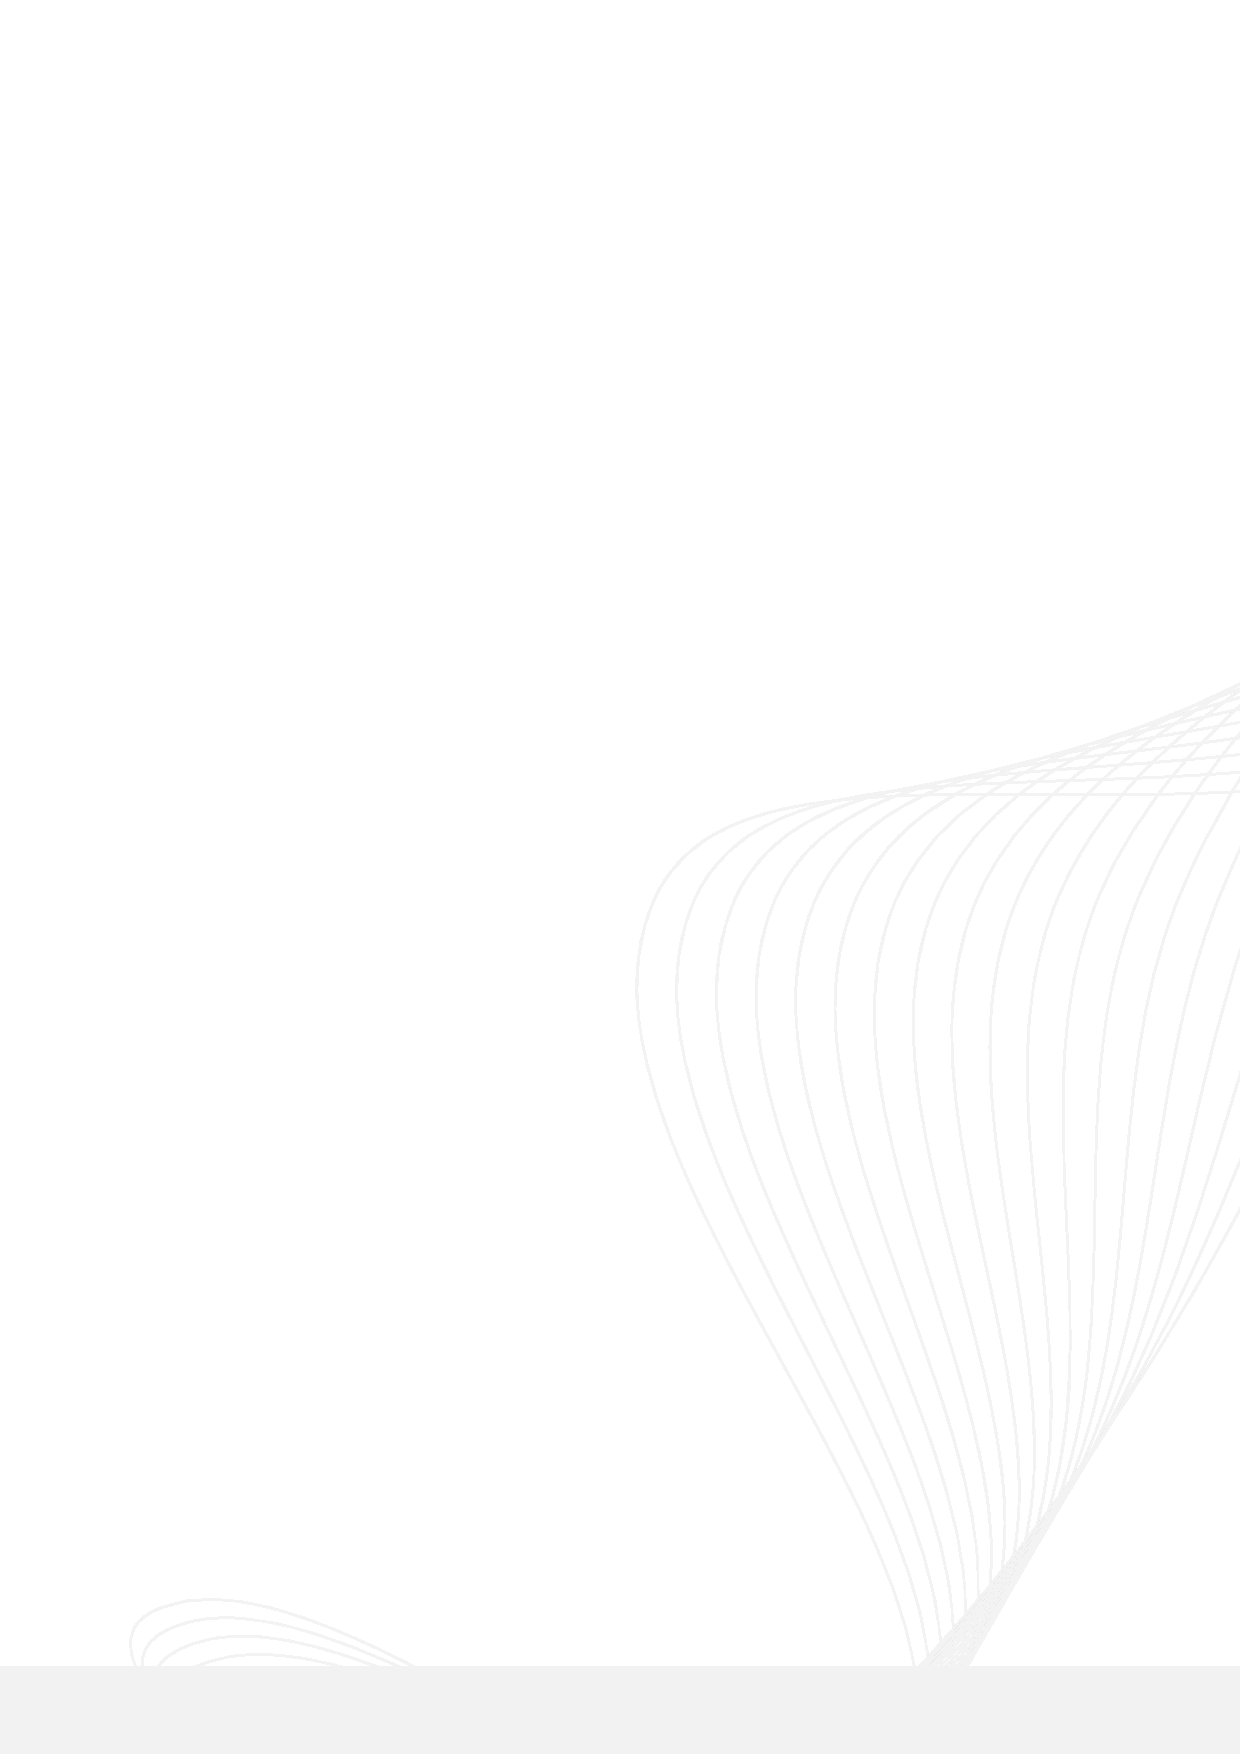
\includegraphics[width=\paperwidth,height=\paperheight,keepaspectratio]{Figures/Theme/Front-Page-BG.pdf}%
    \vfill
    }}}
}

\AddToShipoutPictureBG*{\BackgroundPicCover}

\newgeometry{margin=1.98cm, top=2.15cm, bottom=1.47cm}
\begin{titlepage}
    \latofont
    \ifthenelse{\equal{\CoverOption}{classic}}{\color{white}}{\color{frontpagedark}}
    \vspace*{\baselineskip}

    \ifthenelse{\equal{\CoverOption}{classic}}{
        \ifthenelse{\equal{\SchoolOption}{estg}}{
            \begin{figure}
                
\includegraphics[width=0.485\linewidth]{Figures/Theme/Logotypes/IPLeiria-ESTG-Logo-W.pdf}
            \end{figure}
        }{}
        
        \ifthenelse{\equal{\SchoolOption}{esad}}{
            \begin{figure}
                
\includegraphics[width=0.485\linewidth]{Figures/Theme/Logotypes/IPLeiria-ESAD-Logo-W.pdf}
            \end{figure}
        }{}
        
        \ifthenelse{\equal{\SchoolOption}{esslei}}{
            \begin{figure}
                
\includegraphics[width=0.485\linewidth]{Figures/Theme/Logotypes/IPLeiria-ESSLEI-Logo-W.pdf}
            \end{figure}
        }{}
        
        \ifthenelse{\equal{\SchoolOption}{estm}}{
            \begin{figure}
                
\includegraphics[width=0.485\linewidth]{Figures/Theme/Logotypes/IPLeiria-ESTM-Logo-W.pdf}
            \end{figure}
        }{}
        
        \ifthenelse{\equal{\SchoolOption}{esecs}}{
            \begin{figure}
                
\includegraphics[width=0.485\linewidth]{Figures/Theme/Logotypes/IPLeiria-ESECS-Logo-W.pdf}
            \end{figure}
        }{}
    } {
        \ifthenelse{\equal{\SchoolOption}{estg}}{
            \begin{figure}
%                
\includegraphics[width=0.485\linewidth]{Figures/Theme/Logotypes/IPLeiria-ESTG-Logo-B.pdf}
                % \includegraphics[width=0.4\linewidth]{Figures/Theme/Logotypes/IPLeiria-ESTG-Logo-Old.png}
            \end{figure}
        }{}
        
        \ifthenelse{\equal{\SchoolOption}{esad}}{
            \begin{figure}
                
\includegraphics[width=0.485\linewidth]{Figures/Theme/Logotypes/IPLeiria-ESAD-Logo-B.pdf}
            \end{figure}
        }{}
        
        \ifthenelse{\equal{\SchoolOption}{esslei}}{
            \begin{figure}
                
\includegraphics[width=0.485\linewidth]{Figures/Theme/Logotypes/IPLeiria-ESSLEI-Logo-B.pdf}
            \end{figure}
        }{}
        
        \ifthenelse{\equal{\SchoolOption}{estm}}{
            \begin{figure}
                
\includegraphics[width=0.485\linewidth]{Figures/Theme/Logotypes/IPLeiria-ESTM-Logo-B.pdf}
            \end{figure}
        }{}
        
        \ifthenelse{\equal{\SchoolOption}{esecs}}{
            \begin{figure}
                
\includegraphics[width=0.485\linewidth]{Figures/Theme/Logotypes/IPLeiria-ESECS-Logo-B.pdf}
            \end{figure}
        }{}
    }

    \vspace*{3.5\baselineskip}

    % Title.
	\noindent
    \makebox[\textwidth][l]{%
        \parbox{\dimexpr\textwidth-4cm\relax}{
            \setstretch{1.03}
            \raggedright\bfseries\fontsize{20}{26}\selectfont\GetTitle
        }
    }

    \vspace{0.8\baselineskip}


	\newsavebox{\subtitlebox}
	\sbox{\subtitlebox}{\parbox{\dimexpr\textwidth-7cm\relax}{
			\setstretch{1.03}
			\raggedright\fontsize{14}{19}\selectfont\GetSubtitle
	}}

	\vspace{\ht\subtitlebox}
	
    \vspace{35pt}  

    % Thesis option.
    {\noindent\fontsize{14}{19}\selectfont\GetThesisType}
    
    \vspace{35pt}

    % Author.
    {\noindent\bfseries\fontsize{14}{19}\selectfont\GetFirstAuthor}

    \ifdefined\GetSecondAuthor
        \vspace{8pt}
        {\noindent\bfseries\fontsize{14}{19}\selectfont\GetSecondAuthor}
	\fi

    \ifdefined\GetThirdAuthor
        \vspace{8pt}
        {\noindent\bfseries\fontsize{14}{19}\selectfont\GetThirdAuthor}
	\fi
 
	\vfill

	% University
	{\noindent\fontsize{10}{12}\selectfont\GetUniversity}

    % School.
	{\noindent\fontsize{10}{12}\selectfont\GetSchool}
	
    % Department.
	{\noindent\fontsize{10}{12}\selectfont\GetDepartment}

    % Degree.
	%{\noindent\fontsize{10}{12}\selectfont\GetDegree}

    % Course.
    \ifdefined\GetCourse
        {\noindent\fontsize{10}{12}\selectfont\GetCourse}
	\fi

%    \ifthenelse{\equal{\DocStageOption}{working}}{
%        \vspace{62pt}
%        {\noindent\fontsize{10}{12}\selectfont\overwritecolor{yellow}{\GetDocumentVersion \\ \textit{\today}}} 
%        \vspace{62pt}
%    }{
%        \vspace{125pt}
%    }

	\vspace{25pt}

    % Local & Date.
	{\noindent\fontsize{10}{12}\selectfont\GetDate}

    \vspace{68pt}
\end{titlepage}
\restoregeometry
\MediaOptionLogicBlank
\newcommand\BackgroundPicFrontPage{%
	\put(0,0){%
		\parbox[b][\paperheight]{\paperwidth}{%
			\vfill
			\centering
			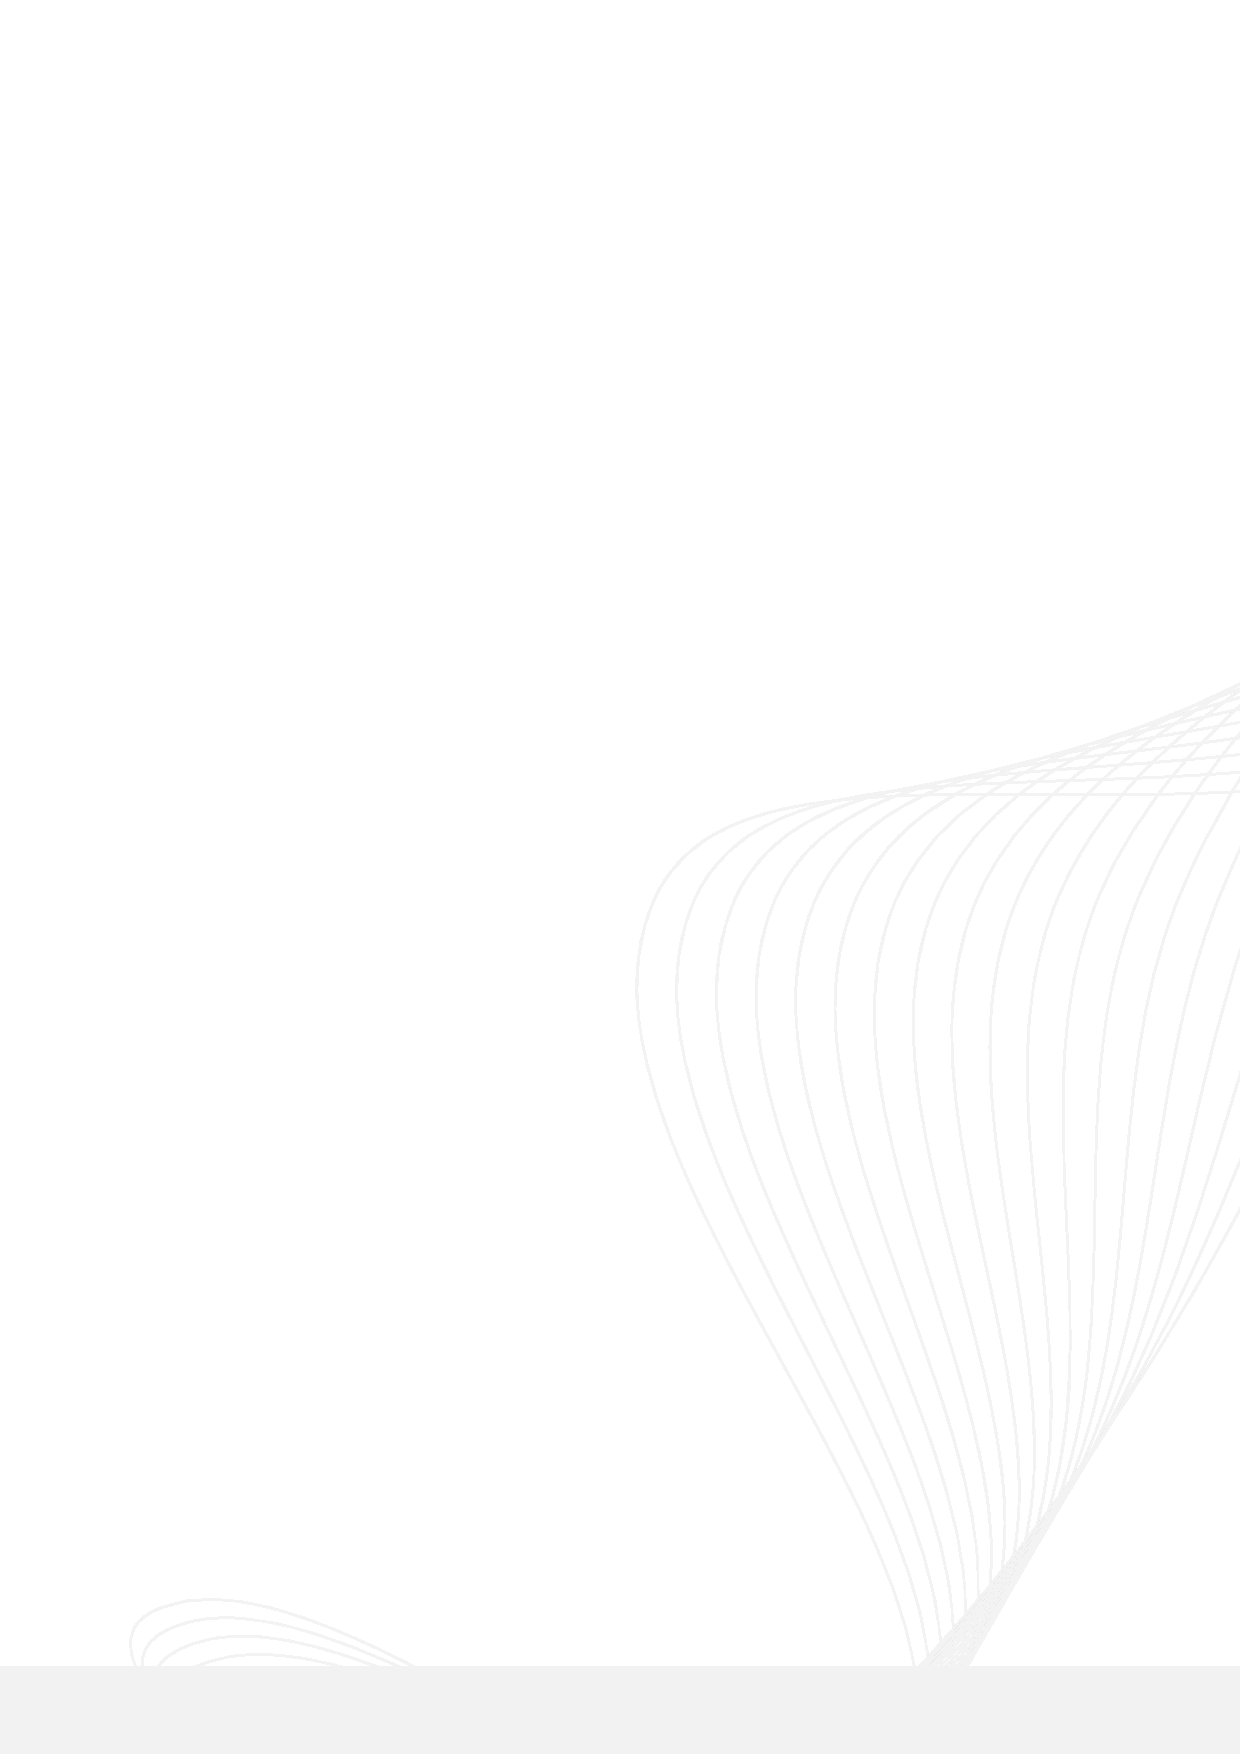
\includegraphics[width=\paperwidth,height=\paperheight,keepaspectratio]{Figures/Theme/Front-Page-BG.pdf}%
			\vfill
		}}}
\AddToShipoutPictureBG*{\BackgroundPicFrontPage}

\newgeometry{margin=1.98cm, top=2.15cm, bottom=1.47cm}
\begin{titlepage}
	\latofont
	\color{frontpagedark}
	\vspace*{\baselineskip}

	%    \begin{figure}
	%%    
\includegraphics[width=0.2\linewidth]{Figures/Theme/Logotypes/TUM-Logo-B.pdf}
	%\end{figure}

	\ifthenelse{\equal{\SchoolOption}{estg}}{
		%        \begin{figure}
		%            
\includegraphics[width=0.485\linewidth]{Figures/Theme/Logotypes/IPLeiria-ESTG-Logo-B.pdf}
		%            % \includegraphics[width=0.4\linewidth]{Figures/Theme/Logotypes/IPLeiria-ESTG-Logo-Old.png}
		%        \end{figure}
	}

	\ifthenelse{\equal{\SchoolOption}{esad}}{
		\begin{figure}
			
\includegraphics[width=0.485\linewidth]{Figures/Theme/Logotypes/IPLeiria-ESAD-Logo-B.pdf}
		\end{figure}
	}

	\ifthenelse{\equal{\SchoolOption}{esslei}}{
		\begin{figure}
			
\includegraphics[width=0.485\linewidth]{Figures/Theme/Logotypes/IPLeiria-ESSLEI-Logo-B.pdf}
		\end{figure}
	}

	\ifthenelse{\equal{\SchoolOption}{estm}}{
		\begin{figure}
			
\includegraphics[width=0.485\linewidth]{Figures/Theme/Logotypes/IPLeiria-ESTM-Logo-B.pdf}
		\end{figure}
	}

	\ifthenelse{\equal{\SchoolOption}{esecs}}{
		\begin{figure}
			
\includegraphics[width=0.485\linewidth]{Figures/Theme/Logotypes/IPLeiria-ESECS-Logo-B.pdf}
		\end{figure}
	}

	\vspace{3.5\baselineskip}

	% Title.
	\noindent
	\makebox[\textwidth][l]{%
		\parbox{\dimexpr\textwidth-4cm\relax}{
			\setstretch{1.03}
			\raggedright\bfseries\fontsize{20}{26}\selectfont\GetTitle
		}
	}

	\vspace{0.8\baselineskip}

	% Subtitle.
	\noindent
	\makebox[\textwidth][l]{%
		\parbox{\dimexpr\textwidth-7cm\relax}{
			\setstretch{1.03}
			\raggedright\fontsize{14}{19}\selectfont\GetSubtitle
		}
	}

	\vspace{35pt}

	% Thesis option.
	{\noindent\fontsize{14}{19}\selectfont\GetThesisType}

	\vspace{35pt}
	% Author.
	{\noindent\bfseries\fontsize{14}{19}\selectfont\GetFirstAuthor}

	%    {\noindent\itshape\fontsize{10}{10}\selectfont Student No. \GetFirstAuthorNumber}

	\ifdefined\GetSecondAuthor
		\vspace{8pt}
		{\noindent\bfseries\fontsize{14}{19}\selectfont\GetSecondAuthor}
	\fi

	\ifdefined\GetThirdAuthor
		\vspace{8pt}
		{\noindent\bfseries\fontsize{14}{19}\selectfont\GetThirdAuthor}
	\fi

	\vfill

	{
		\noindent
		\latofont
		\fontsize{10}{12}\selectfont
		\renewcommand{\arraystretch}{0.1}
		\hspace*{-2.5pt}\begin{tabular}{@{}r@{\hspace{5pt}}>{\raggedright\arraybackslash}m{6cm}@{}}
			\textbf{Supervisor:}      & \GetSupervisor                                                                 \\ [-.7ex]
			                          & \setstretch{0.9}{\fontsize{8}{10}\selectfont\itshape \GetSupervisorChair}      \\ [.5ex]

			\ifdefined\GetAdvisor
			\textbf{Advisor:}         & \GetAdvisor                                                                    \\ [-.7ex]
			                          & \setstretch{0.9}{\fontsize{8}{10}\selectfont\itshape \GetAdvisorChair}         \\ [.5ex]
			\fi

			\ifdefined\GetCoSupervisor
			\textbf{Co-supervisor:}   & \GetCoSupervisor                                                               \\ [-.7ex]
			                          & \setstretch{0.9}{\fontsize{8}{10}\selectfont\itshape \GetCoSupervisorTitle}    \\ [.5ex]
			\fi
			\textbf{Date:} & 15.09.2025                                                                     \\ [-.7ex]

			\ifdefined\GetSecCoSupervisor
			                          & \GetSecCoSupervisor                                                            \\ [-.7ex]
			                          & \setstretch{0.9}{\fontsize{8}{10}\selectfont\itshape \GetSecCoSupervisorTitle} \\
			\fi
		\end{tabular}
	}

	\vspace{58pt}

	% University
	{\noindent\fontsize{10}{12}\selectfont\GetUniversity}

	% School.
	{\noindent\fontsize{10}{12}\selectfont\GetSchool}

	% Department.
	{\noindent\fontsize{10}{12}\selectfont\GetDepartment}

	% Degree.
	%{\noindent\fontsize{10}{12}\selectfont\GetDegree}

	% Course.
	\ifdefined\GetCourse
	{\noindent\fontsize{10}{12}\selectfont\GetCourse}
	\fi

	\vspace{25pt}

	% Local and date.
	{\noindent\fontsize{10}{12}\selectfont\GetDate}

	\vspace{68pt}
\end{titlepage}
\restoregeometry
\MediaOptionLogicBlank

%%% Copyright Statement %%%
\pagenumbering{gobble} % Prevent page numbering.

\vspace*{\fill}

\noindent I confirm that this bachelor's thesis is my own work and I have documented all sources and material used.

\vspace*{\fill}

\noindent Munich, September 15\textsuperscript{th}, 2025\hfill Niklas Ladurner

\MediaOptionLogic

%%% Roman Numeration %%%
\pagenumbering{roman}

%%% Acknowledgements %%%
\chapter*{Acknowledgements}

{
	\setlength\parindent{0pt}
	% Manish
	I would like to express my deepest gratitude to my advisor Manish Mishra. His guidance, patience, and insightful explanations during our meetings were invaluable in helping me understand AutoPas and its wide array of complex features. His continuous encouragement and his in-depth analysis of preliminary results pushed me to refine my ideas and improve the quality of this thesis.
	\vspace*{\baselineskip}
	
	% Friends
	Additionally, I would like to thank all my friends who kindly took the time to proofread parts of this work and provide thoughtful feedback. Their constructive criticism and suggestions helped shape this thesis into what it is now.
	\vspace*{\baselineskip}
	
	% LRZ
	The evaluation of our proposed mechanisms could not have been performed without sizeable processing capabilities. Thus, for supporting this thesis by providing computing time on its Linux-Cluster, I gratefully acknowledge the Leibniz Supercomputing Centre.
	\vspace*{\baselineskip}
	
	% template
	Lastly, I want to thank José Areia and all contributors to the \textit{IPLeiria-Thesis}\footnote{\href{https://github.com/joseareia/ipleiria-thesis}{https://github.com/joseareia/ipleiria-thesis}} template, which was adapted and used in this work.
}


\MediaOptionLogicBlank

%%% Abstract %%%
\thispagestyle{plain}

\pdfbookmark[1]{Abstract}{abstract}
\chapter*{Abstract}

Particle simulations have become an indispensable tool in research and are used across a wide range of applications. Depending on the specific scenario, different simulation configurations may be more suitable. AutoPas is a particle simulation library that offers a simple black-box interface for researchers. To achieve this, AutoPas reevaluates the optimal configuration at fixed intervals. This thesis proposes a dynamic approach to determine ideal points for the initiation of new tuning phases.

% TODO: add results and rewrite

\MediaOptionLogicBlank

\chapter*{Zusammenfassung}

TODO

\MediaOptionLogicBlank

%%% AI Acknowledgement %%%
\ifthenelse{\equal{\AiAckOption}{true}}{%
    \ifthenelse{\equal{\LanguageOption}{portuguese}}{%
        \chapter*{Declaração sobre o Uso de Inteligência Artificial}

        \guideinfo{É uma boa prática académica indicar brevemente como, porquê e quando a IA foi utilizada. Explicar as ações tomadas e as razões que lhes estão subjacentes promove a reflexão crítica, aprofunda a compreensão do papel da IA na aprendizagem e ajuda a avaliar o seu impacto na qualidade e integridade do trabalho. Esta página pode ser removida definindo a opção \texttt{aiack} como \texttt{false} nas opções da classe do documento.}
    
        \vspace{2em}
        
        \exampleinfo{%
        Reconheço a utilização do ChatGPT (\url{https://chatgpt.com}) para aperfeiçoar o tom académico e melhorar a precisão linguística deste trabalho, incluindo aspectos de gramática, pontuação e vocabulário.
        
        \vspace{1em}
        
        \noindent\textbf{Descrição da Utilização}
        
        \prompt[1]{Num parágrafo, descreva simplesmente o que é o LaTeX.}
        
        \aioutput[1]{O LaTeX é um sistema de composição de alta qualidade, normalmente utilizado para produzir documentos científicos e matemáticos, devido ao seu poderoso manuseamento de fórmulas e bibliografias. Ao contrário dos processadores de texto, utiliza ficheiros de texto simples com etiquetas de marcação para definir a estrutura e a formatação de um documento, permitindo um controlo preciso da disposição e do aspeto. É especialmente popular no meio académico e na investigação para a criação de teses, artigos de revistas e apresentações.}
        }
    }{%
        \chapter*{AI Acknowledgement}

        \guideinfo{It is good academic practice to briefly state how, why, and when AI was used. Explaining both the actions taken and the reasons behind them encourages critical reflection, deepens understanding of AI's role in learning, and supports the evaluation of its impact on your work’s quality and integrity. This page can be removed by setting the option \texttt{aiack} to \texttt{false} in the document class options.}

        \vspace{2em}
        
        \exampleinfo{%
        I acknowledge the use of ChatGPT (\url{https://chatgpt.com}) to refine the academic tone and improve the linguistic accuracy of this work, including aspects of grammar, punctuation, and vocabulary.
        
        \vspace{1em}
        
        \noindent\textbf{Description of Use}
        
        \prompt[1]{In a paragraph, simply describe what LaTeX is.}
        
        \aioutput[1]{LaTeX is a high-quality typesetting system commonly used for producing scientific and mathematical documents due to its powerful handling of formulas and bibliographies. Unlike word processors, it uses plain text files with markup tags to define the structure and formatting of a document, allowing precise control over layout and appearance. It is especially popular in academia and research for creating theses, journal articles, and presentations.}
        }
    }
    
    \MediaOptionLogicBlank   
}{}

%%% Table of Contents, List of Figures and List of Tables %%%
\bookmarktocentry\tableofcontents
\listoffigures
\listoftables

%%% Print: Glossary and Acronyms %%%
%\glossarytoc\printnormalglossary
%\acronymtoc\printacronymglossary
%\symboltoc\printsymbolglossary

%%% Arabic Numeration %%%
\pagenumbering{arabic}

%%% Chapters (**Insert Yours Here**) %%%
\chapter[Introduction]{Introduction}
\label{cp:introduction}

{
	\parindent0pt
	This chapter introduces some fundamental concepts necessary to understand Molecular Dynamics (MD) simulations. We begin with a discussion of the motivation behind the general $n$-body problem and the goals of this thesis in \autoref{sec:motivation}.
	
	Afterwards, the components of a simple MD simulation loop are presented in \autoref{sec:md}. These include Newton’s laws of motion for providing the governing equations of particle trajectories, the Lennard-Jones potential as a model for pairwise interactions, and the Störmer-Verlet algorithms as a numerical scheme for integrating the equations of motion.
}


% TODO: check atomic/molecular interactions

\section{Motivation}
\label{sec:motivation}

The $n$-body problem is a foundational challenge of classical physics. It  concerns the interaction and movement of bodies, like the trajectories of masses in the solar system. At such astronomic scales, general relativity additionally introduces a high degree of complexity. Yet, even in classical Newtonian physics, the systems of equations tend to no longer be solvable by analytic means if $n>2$ bodies are involved, except for certain special cases. Hence, numerical algorithms have become essential in finding approximate solutions. \cite{Arnold1985}

With the advent of computer-based simulation, the feasibility of numerical solutions to the $n$-body problem has increased significantly.
Over the past few decades, advances in high performance computing (HPC) have further increased both scale and efficiency of such simulations, allowing for the modeling of large systems at unprecedented resolution. For instance, the TianNu project simulated \num{2.97e12} particles in 2017 on the Tianhe-2 supercomputer \cite{Emberson2017}.
These days, particle simulations have established themselves as indispensable tools across a wide range of scientific fields. Applications reach from drug discovery \cite{Hollingsworth2018} to plasma physics \cite{Verboncoeur2005} and materials science \cite{Parteli2016}.

One example of a software framework enabling $n$-body simulations is the AutoPas library \cite{Gratl2019}. Its internal mechanisms will be discussed in detail in \autoref{cp:autopas}; for the motivation of this thesis it suffices to know, that AutoPas seeks to dynamically select optimal simulation configurations without requiring expert knowledge during setup (\enquote{autotuning}).

To achieve this, so-called tuning phases are initiated at fixed intervals. During each tuning phase, different configurations are sampled for a predetermined number of iterations, after which the best performing configuration is selected to simulate the remaining iterations until the next tuning phase. Naturally, these static intervals do not necessarily align with the points at which it would be most advantageous to switch configurations. Consider a scenario, in which the optimal configuration changes rapidly in the beginning, but stabilizes and settles into an equilibrium later on. Having one uniform static interval, it would be either too short -- resulting in unnecessary tuning phases during equilibrium, or too long -- resulting in suboptimal performance in the early phase.

This thesis proposes a method to resolve this problem by dynamically initiating tuning phases based on live simulation data.

% TODO: dynamic intervals figure?

\section{Molecular Dynamics}
\label{sec:md}
% quantum behaviour
Molecular Dynamics (MD) simulation is one method of solving the classical $n$-body problem on the molecular level. At that level, the interactions between atoms are subject to the of laws quantum mechanics, in particular the Schrödinger equation. That equation however is unsuitable for the simulation of larger systems due to its complexity by nature of being a partial differential equation.

Therefore, simplifications such as the Born-Oppenheimer approximation have to be employed. This approximation is based on the fact that the nuclei of atoms have much greater mass than the electrons surrounding them. Under the additional assumption, that the nuclei can be considered static relative to the movements of the electrons, we can separate the Schrödinger equation into two parts coupled by an interaction potential. Using further simplifications, we obtain \eqref{eq:born_oppenheimer}, which directly corresponds to the classical laws of motion as stated by Newton (cf. \autoref{sec:newton}). In this equation, $\vb p_i(t), \vb a_i(t), m_i, V\left(\vb p_i(t)\right)$ are the position, acceleration, mass and potential acting on a particle $i$ at time $t$. \cite{Born1927, Voorhis2005, Griebel2007} 

\begin{equation}
	m_i\vb a_i(t) = -\nabla_{\vb p_i} V\left(\vb p(t)\right)\label{eq:born_oppenheimer}
\end{equation}

The simplest interatomic potentials one could apply here describe the interactions between only two particles, such as the Gravitational, Lennard-Jones or Coloumb potentials. \cite{Griebel2007}

Considering the formula presented in \eqref{eq:born_oppenheimer}, the main MD simulation loop is rather simple. It consists of calculating the forces between particles or atoms and integrating the equations of motion. These two steps are repeated until an equilibrium is reached, at which point the desired measurements can be taken. \cite{Frenkel2002}





\subsection{Newton's laws of motion}
\label{sec:newton}
As referred to before, Newton's laws of motion can be applied to MD simulation in approximating particle behavior. These well-known laws of classical mechanics are as follows. \cite{Newton1934}
\begin{enumerate}[label=\Roman*.]
	\item \textit{Every object perseveres in its state of rest, or of uniform motion in a right line, unless it is compelled to change that state by forces impressed thereon.}

	      In other words, if the net force on any body is zero, its velocity is constant.
	\item \textit{The alteration of motion is ever proportional to the motive force impressed; and is made in the direction of the right line in which that force is impressed.}

	      In other words, $F=m\cdot a$.
	\item \textit{To every action there is always opposed an equal reaction: or, the mutual actions of two bodies upon each other are always equal, and directed to contrary parts.}

	      In other words, if one body exerts force $F_a$ on another body, than the second body exerts force $F_b=-F_a$ on the first body.
\end{enumerate}

The second law is of utmost importance, as it allows to compute trajectories of particles based on the force acting upon them. The third law, while secondary in dynamics, is useful especially regarding optimizations: for pairwise interactions, the force needs to be evaluated only once, since the second particle experiences a force of the same magnitude in opposed direction. \cite{Gratl2021}

% TODO: ref to Newton3 optimization

\subsection{Lennard-Jones Potential}
\label{sec:lj_potential}
Simulating all pairwise interactions between atoms has complexity $\mathcal{O}\left(n^2\right)$. To reduce this complexity, most MD simulations restrict themselves to short-range interactions. As the forces of these interactions are negligible if the interacting particles are far apart, a cutoff-radius can be introduced after which the forces can be assumed to be close to zero. This significantly reduces the computational complexity, as only the interactions between close neighbors have to be computed. \cite{Gratl2021}

The Lennard-Jones (LJ) potential is one such short-range interaction potential that acts on pairs of particles. It is based on empirical data and a sufficiently good approximation such that macroscopic effects can be derived from simulating the interactions at an atomic level.
It is most frequently used in the form of the 12-6 potential as defined in \eqref{eq:lj_12_6}.

\begin{equation}
	V_{\text{LJ}}(r)=4\varepsilon\left[\left(\frac{\sigma}{r}\right)^{12}-\left(\frac{\sigma}{r}\right)^{6}\right]\label{eq:lj_12_6}
\end{equation}

In this equation, $r$ is the distance between the two particles, $\varepsilon$ the interaction strength and $\sigma$ the distance at which the potential signs change (zero-crossing). Parameters $\varepsilon, \sigma$ are dependent on the simulation context, e.g. the material which ought to be simulated. The potential function is illustrated in \autoref{fig:lj_graph}. \cite{Wang2020, Lenhard2024}


\begin{figure}[htpb]
	\centering
	\begin{tikzpicture}
		\begin{axis}[height=0.4\textwidth, width=0.6\textwidth,
			xmin = 0.75,
			xmax = 3.25,
			ymin = -1.25,
			ymax = 2.25,
			xlabel={Distance $r$ between particles},
			ylabel={Potential $V_{\text{LJ}}$},
			xtick={{2^(1/6)},1.5,2,2.5,3},
			xticklabels={$r_\text{min}$,1.5$\sigma$,2$\sigma$,2.5$\sigma$,3$\sigma$},
			ytick={-1, 0, 1, 2},
			yticklabels={$-\varepsilon$,0,$\varepsilon$,2$\varepsilon$},
			clip=false]
			\addplot [
				color=chaptertumblue, very thick,
				domain=0.95:3,
				samples=400,
			]
			{4*((1/x)^(12) - (1/x)^6)};
			\draw[black!80] (axis cs:0.75,0) -- (axis cs:3.25,0);
			\draw[black!80] (axis cs:{2^(1/6)},2.25) -- (axis cs:{2^(1/6)},-1.25);
			\draw[black!80, dashed] (axis cs:0.75,-1) -- (axis cs:{2^(1/6)},-1);
			\draw [decorate,decoration={brace, amplitude=1ex, raise=0.5ex}] (axis cs:0.75,2.25) -- (axis cs:{2^(1/6)-0.0125},2.25) node[midway, yshift=2.5ex]{Attraction\vphantom{p}};
			\draw [decorate,decoration={brace, amplitude=1ex, raise=0.5ex}] (axis cs:{2^(1/6)+0.0125},2.25) -- (axis cs:3.25,2.25) node[midway, yshift=2.5ex]{Repulsion};
		\end{axis}
	\end{tikzpicture}
	\caption{An illustration of the potential well of the 12-6 LJ potential, with the minimum of $-\varepsilon$ at $r_\text{min}=\sigma\sqrt[6]{2}$ and zero-crossing at $\sigma$. The figure is based on Lenhard et al. \cite{Lenhard2024}}
	\label{fig:lj_graph}
\end{figure}

% TODO: mark r=1\sigma as zero-crossing point

\subsection{Störmer-Verlet Algorithm}
\label{sec:stoermer_verlet}
Using LJ potentials and Newton's laws of motion, we can construct a system of ordinary differential equations. To solve them analytically is practically infeasible for large systems, therefore numeric solvers have to be used in approximating a solution, as stated before.

% TODO: symplectic integrator, good macroscopic simulation
The Störmer-Verlet algorithm is one such numeric technique for solving the systems constructed as mentioned.
With $\vb p_i(t), \vb v_i(t), \vb a_i(t), m_i, \vb F_i(t)$ as the position, velocity, acceleration, mass and force acting on a particle $i$ at time $t$, we can derive the algorithm by the summation of Taylor expansions. First, we deduce the position of particle $i$ at time $t+\delta t$, as in \eqref{eq:pos_taylor_forward}. Secondly, we take a backwards step to $t-\delta t$, as in \eqref{eq:pos_taylor_backward}.
\begin{equation}
	\vb p_i(t+\delta t) = \vb p_i(t)+\delta t\dot{\vb p}_i(t)+\frac{1}{2}\delta t^2\ddot{\vb p}_i(t)+\frac{1}{6}\delta t^3\dddot{\vb p}_i(t)+\mathcal{O}(\delta t^4)\label{eq:pos_taylor_forward}
\end{equation}
\begin{equation}
	\vb p_i(t-\delta t) = \vb p_i(t)-\delta t\dot{\vb p}_i(t)+\frac{1}{2}\delta t^2\ddot{\vb p}_i(t)-\frac{1}{6}\delta t^3\dddot{\vb p}_i(t)+\mathcal{O}(\delta t^4)\label{eq:pos_taylor_backward}
\end{equation}

By adding both \eqref{eq:pos_taylor_forward} and \eqref{eq:pos_taylor_backward} and reordering terms, we conclude \eqref{eq:pos_verlet}.
\begin{equation}
\vb p_i(t+\delta t) = 2\vb p_i(t) - \vb p_i(t-\delta t) + \delta t^2\ddot{\vb p}_i(t) + \mathcal{O}(\delta t^4)\label{eq:pos_verlet}
\end{equation}

As the second derivative of the position $\vb p_i(t)$ is the acceleration $\vb a_i(t)$, we can express \eqref{eq:pos_verlet} as \eqref{eq:acc_verlet}. Where, by Newton's second law, $\vb a_i(t) = \frac{\vb F_i(t)}{m_i}$.
\begin{equation}
	\vb p_i(t+\delta t) = 2\vb p_i(t) - \vb p_i(t-\delta t) + \delta t^2{\vb a}_i(t) + \mathcal{O}(\delta t^4)\label{eq:acc_verlet}
\end{equation}

By this formulation we could already calculate the velocities of the particles, however, there are some drawbacks -- e.g. high error propagation. A more exact and efficient approach, sometimes referred to as the Velocity-Verlet algorithm, can be derived similarly.
For that, considering \eqref{eq:velocity}, we can rearrange and substitute into \eqref{eq:pos_verlet} to conclude \eqref{eq:verlet_pos2} and finally \eqref{eq:verlet_vel}.
\begin{equation}
	\vb v_i(t) = \frac{\vb p_i(t+\delta t) -\vb p_i(t-\delta t)}{2\delta t} \rightsquigarrow \vb p_i(t-\delta t)= \vb p_i(t+\delta t)-2\delta t \vb v_i(t) \label{eq:velocity}
\end{equation}

\begin{equation}
	\vb p_i(t+\delta t) = \vb p_i(t) +\delta t \vb v_i(t) + \frac{\delta t^2}{2}{\vb a}_i(t) + \mathcal{O}(\delta t^4) \label{eq:verlet_pos2}
\end{equation}
\begin{equation}
	\vb v_i(t+\delta t) = \vb v_i(t)+\frac{\delta t}{2}\left[\vb a_i(t)+ \vb a_i(t+\delta t)\right] + \mathcal{O}(\delta t^4) \label{eq:verlet_vel}
\end{equation}
Because of the aforementioned improved properties of this method, it is often preferred in MD simulations. \cite{Fulst2013, Leimkuhler2005, Hairer2003}

% TODO: refer to experiments done in md-flexible
% md-flexible is a simple molecular dynamics simulation built around AutoPas. It simulates the Lennard-Jones 12-6 potential on single-site particles with Störmer- Verlet time integration. 




\chapter[AutoPas]{AutoPas}
\label{cp:autopas}

{
	\parindent0pt
	This chapter examines the particle simulation library AutoPas and provides an overview of its architecture and features. In \autoref{sec:background}, the concept of autotuning is introduced, as well as the \texttt{md-flexible} application. %TODO ?
	The various algorithmic configuration parameters available  are introduced thereafter in \autoref{sec:config_params}. Additionally, \autoref{sec:tuning_strategies} shortly outlines the different tuning strategies for the selection of the optimal combination of these parameters.

	The contents of this chapter are mainly drawn from the works introducing AutoPas, specifically the publications by Gratl et al. \cite{Gratl2019, Gratl2021, GratlGassner2025} and Seckler et al. \cite{Seckler2021}, as well as the AutoPas documentation \cite{AutoPas2025}.
}


\section{Background}
\label{sec:background}
AutoPas is an open-source \CC{} library that facilitates short-range MD simulations. The feature that sets AutoPas apart from other particle simulation software such as LAMMPS\footnote{\href{https://www.lammps.org/}{https://www.lammps.org/}}, ls1-mardyn\footnote{\href{https://www.ls1-mardyn.de/}{https://www.ls1-mardyn.de/}} or GROMACS\footnote{\href{https://www.gromacs.org/}{https://www.gromacs.org/}}, is the autotuning algorithm.

The aforementioned programs are highly specialized on specific applications and therefore focus on optimizing the algorithms used in these environments.
AutoPas, on the other hand, tries to provide optimal simulation conditions for a broader range of scenarios by implementing a wide selection of algorithms and switching between them at runtime.
This removes the need for expert knowledge in simulation setup and allows for a simple interface through which the AutoPas library can be viewed as a black-box.

As referred to earlier, this autotuning approach is currently implemented as follows: In each iteration that is a multiple of a predefined \texttt{tuning-interval}, a tuning phase is initiated. In these tuning phases, a number of configurations are selected to be sampled. These configurations each represent a distinct combination of algorithmic settings (c.f. \autoref{sec:config_params}). Each configuration is sampled, i.e. executed for a set number of iterations, after which the measurements are condensed into a single value, referred to as \enquote{evidence}. This evidence is used to rank the sampled configurations based on a tuning metric; either run time or energy consumption. The best configuration is selected to compute the subsequent iterations until the beginning of the next tuning phase.

%TODO: Duplication of Motivation

As AutoPas is only a library, we require an application that interacts with it and provides a front end to allow for our particle simulations. In this work, we will use the \texttt{md-flexible} application, provided together with AutoPas. Based on the LJ potential, \texttt{md-flexible} facilitates MD simulations with integrated parallelization, shared memory computation, load balancing, and highly configurable scenario generators.
% Autotuning


% TODO: explain configs in Background, remove duplications in other sections?

\section{Configuration Parameters}
\label{sec:config_params}

As outlined in \autoref{sec:background}, AutoPas is designed to allow for dynamic adaptation of the algorithmic configuration used in computing the actual simulation steps. The relevant parameters are categorized and described in the following.

\subsection{Containers}

Containers in AutoPas are classes responsible for particle management and neighbor identification. They store the actual particle data in a specific memory layout and allow for the efficient lookup of neighbors, i.e. particles inside the cutoff radius $r_c$. Grouped by neighbor identification algorithm, there are currently four different types of containers.

\begin{description}[leftmargin=!,labelwidth=\widthof{\textbf{Verlet Cluster Lists}}]
	\item[\textbf{Direct Sum}] The simplest algorithm is the direct sum: It calculates the distances between the current particle and all other particles, discards those which lie outside of $r_c$, and proceeds with the force calculations on the remaining particles. As this method has complexity $\mathcal{O}\left(n^2\right)$, it is only suitable for small scenarios.
	\item[\textbf{Linked Cells}] The linked cell approach divides the simulation space up into cells along a regular grid. Each particle is then assigned to the cell corresponding to its location in space. Considering a cell size greater or equal to $r_c$, only neighboring cells have to be considered in the force calculations. For homogeneous particle distributions, this reduces the complexity to $\mathcal{O}\left(n\right)$. Additionally, particles close to each other in simulation space are close in memory, which results in cache-friendly behavior and allows for vectorization.
	\item[\textbf{Verlet Lists}] One drawback of the linked cells algorithm is the high number of particles that lie inside neighboring cells, but outside the cutoff radius. They are discarded in the force computation, but still require the distance computations. The Verlet list algorithm solves this issue by introducing a neighbor list of interaction partners for each particle. As rebuilding these lists is expensive, not only neighbors inside the cutoff radius are stored, but also particles that might come into interaction range. This is achieved by extending the radius by a so-called Verlet skin. As particles move, these neighbor lists have to be rebuilt periodically, relying on other neighbor identification algorithms such as linked cells. Furthermore, Verlet lists have a large memory footprint (one list per particle) and do not provide the advantageous memory properties of linked cells.
	\item[\textbf{Verlet Cluster Lists}] To reduce the overall number of lists in the Verlet list approach, multiple particles can be clustered together, effectively combining their individual neighbor lists to a single one for the whole cluster. This is possible due to the fact that neighboring particles are likely to share multiple of their neighbors. The clustering is based on a subdivision of the simulation domain into a Cartesian grid ($x/y$) which, extruded along the third dimension ($z$), forms several towers. Inside each of these towers, particles are grouped into clusters of size $M$, ordered by their position along the $z$-axis. Instead of an exact combination of all cutoff radii, a simple bounding box is constructed around each cluster. Thus, Verlet cluster lists not only reduce the total number of neighbor lists, but also allow for vectorization, as clusters are groupings of spatially close particles. On the other hand, the number of particles for which distance calculations have to be performed increases.
\end{description}

\begin{figure}
	\centering
	\caption{A comparison of the different Containers implemented in AutoPas [TODO]}
	\label{fig:containers}
\end{figure}

\subsection{Traversals}
\label{sec:traversals}
Containers provide an efficient way to identify neighbors of a particle --- to efficiently compute the interactions themselves however, the traversal, i.e. the order in which particles are iterated over, is equally important. Traversals are relevant for the performance mostly due to memory and cache access patterns. Different container types require traversals, tailored to the data structures used in storing the neighbors. A small selection of these traversals will be explained hereafter.

%TODO:
\begin{description}[leftmargin=!,labelwidth=\widthof{\textbf{VL List Iteration}}]
\item[\textbf{C01}] TODO
\item[\textbf{VL List Iteration}] TODO
\item[\textbf{LC C04}] TODO
\end{description}

\subsection{Additional Parameters}
Moreover, there are a number of additional configuration parameters that do not fall into the aforementioned groups. They are given below.

\begin{description}[leftmargin=!,labelwidth=\widthof{\textbf{Cell Size Factor}}]
	\item[\textbf{Data Layout}] The data layout option concerns the layout of the particle structures in memory. As each particle has multiple attributes associated to it, all particles together can be laid out either as an Array of Structures (AoS) or a Structure of Arrays (SoA). In the AoS layout, all particles are stored after each other; in the SoA layout, each attribute type is stored in a separate array, with each entry holding the value for a specific particle. \autoref{fig:aos_soa} illustrates both principles.
	\item[\textbf{Newton3}] As mentioned in \autoref{sec:newton}, Newton's third law states that $F_a = -F_b$ for two bodies $a, b$ exerting forces on each other. This allows for optimizing pairwise interactions, as only one force has to be computed. However, this approach is not always beneficial as it may limit parallelization --- once the force is evaluated, both particles must be updated at once.
	\item[\textbf{Cell Size Factor}] The cell size factor (CSF) parameter specifies the side length of the cells in relation to the interaction cutoff radius $r_c$<. It can reduce the number of particles for which distances have to be calculated, as a smaller cell side length better approximates the spherical nature of the cutoff radius. This behavior is illustrated in  \autoref{fig:lc_csf}.
\end{description}


\begin{figure}

	\def\sz{2em}
	\def\rc{4em}
	\def\psz{0.4em}
	\tikzset{
		mgrid/.style = {matrix of nodes, ampersand replacement=\&, nodes={draw, minimum width=\sz, minimum height=\sz, anchor=center}, column sep=-\pgflinewidth, row sep=-\pgflinewidth},
		particle/.style={draw=black, circle, minimum size=\psz, inner sep=0pt, outer sep = 0pt},
		particleOutside/.style={particle, fill=violet, pattern={Lines[angle=45,distance=1pt]}},
		particleInside/.style={particle, fill=green, pattern=dots},
		checked/.style={draw=none, fill=tumblueaccverylight, inner sep=0pt},
		checkedborder/.style={draw=chaptertumblue, very thick, inner sep = 0pt},
		cutoff/.style={draw=chaptertumblue, circle, very thick, dashed, minimum size=\rc, inner sep=0pt, outer sep=0pt},
		arrow/.style={-latex},
	}
	\begin{subfigure}{0.5\textwidth}
		\centering
		\begin{tikzpicture}
			\draw[step=\sz] (0,0) grid (5*\sz,5*\sz);


			\begin{scope}[on background layer]
				\node[checked, fit={(1*\sz,1*\sz) (4*\sz,4*\sz)}] {};
			\end{scope}

			\node[checkedborder, fit={(1*\sz,1*\sz) (4*\sz,4*\sz)}] {};


			\node[particle, fill=lightred] (pact) at (2.5*\sz+0.2em,2.5*\sz-0.2em) {};
			\node[cutoff] (cr) at (pact) {};

			\node[particle]        (p1)  at (1.5*\sz+0.3em,4.5*\sz-0.3em) {};
			\node[particle]        (p2)  at (4.5*\sz-0.6em,2.5*\sz-0.4em) {};
			\node[particle]        (p3)  at (0.5*\sz+0.6em,3.5*\sz-0.6em) {};
			\node[particleInside]  (p4)  at (2.5*\sz+0.1em,1.5*\sz+0.4em) {};
			\node[particle]        (p5)  at (3.5*\sz-0.5em,0.5*\sz+0.5em) {};
			\node[particle]        (p6)  at (4.5*\sz-0.3em,4.5*\sz-0.4em) {};
			\node[particleOutside] (p7)  at (3.5*\sz-0.7em,3.5*\sz+0.6em) {};
			\node[particleInside]  (p8)  at (1.5*\sz+0.5em,2.5*\sz-0.67em) {};
			\node[particle]        (p9)  at (0.5*\sz-0.2em,0.5*\sz+0.3em) {};
			\node[particle]        (p10) at (4.5*\sz+0.7em,1.5*\sz-0.7em) {};
			\node[particleOutside] (p11) at (1.5*\sz+0.5em,3.5*\sz+0.4em) {};
			\node[particle]        (p12) at (2.5*\sz-0.6em,0.5*\sz+0.7em) {};
			\node[particle]        (p13) at (3.5*\sz+0.7em,4.5*\sz-0.1em) {};
			\node[particle]        (p14) at (0.5*\sz+0.4em,2.5*\sz-0.2em) {};
			\node[particleOutside] (p15) at (1.5*\sz+0.2em,1.5*\sz-0.5em) {};
			\node[particleInside]  (p16) at (2.5*\sz+0.4em,3.5*\sz-0.5em) {};
			\node[particleOutside] (p17) at (1.5*\sz-0.6em,2.5*\sz+0.5em) {};
			\node[particleOutside] (p18) at (3.5*\sz+0.7em,1.5*\sz+0.2em) {};
			\node[particleInside]  (p19) at (3.5*\sz-0.5em,2.5*\sz+0.7em) {};
			\node[particleOutside] (p20) at (3.5*\sz-0.4em,1.5*\sz-0.7em) {};




			\draw[arrow] (pact) -- (p11);
			\draw[arrow] (pact) -- (p16);
			\draw[arrow] (pact) -- (p7);
			\draw[arrow] (pact) -- (p8);
			\draw[arrow] (pact) -- (p17);
			\draw[arrow] (pact) -- (p19);
			\draw[arrow] (pact) -- (p15);
			\draw[arrow] (pact) -- (p4);
			\draw[arrow] (pact) -- (p18);
			\draw[arrow] (pact) -- (p20);


		\end{tikzpicture}
	\end{subfigure}%
	\begin{subfigure}{0.5\textwidth}
		\centering
		\begin{tikzpicture}
			\def\sz{2em}
			\matrix[mgrid] (mat) at (0,0) {
			{}\&{}\&{}\&{}\&{}\\
			{}\&{}\&{}\&{}\&{}\\
			{}\&{}\&{}\&{}\&{}\\
			{}\&{}\&{}\&{}\&{}\\
			{}\&{}\&{}\&{}\&{}\\
			};
			%			\def\sz{1em}
			%			\matrix[mgrid] (mat) {
			%			{}\&{}\&{}\&{}\&{}\&{}\&{}\&{}\&{}\&{}\\
			%			{}\&{}\&{}\&{}\&{}\&{}\&{}\&{}\&{}\&{}\\
			%			{}\&{}\&{}\&{}\&{}\&{}\&{}\&{}\&{}\&{}\\
			%			{}\&{}\&{}\&{}\&{}\&{}\&{}\&{}\&{}\&{}\\
			%			{}\&{}\&{}\&{}\&{}\&{}\&{}\&{}\&{}\&{}\\
			%			{}\&{}\&{}\&{}\&{}\&{}\&{}\&{}\&{}\&{}\\
			%			{}\&{}\&{}\&{}\&{}\&{}\&{}\&{}\&{}\&{}\\
			%			{}\&{}\&{}\&{}\&{}\&{}\&{}\&{}\&{}\&{}\\
			%			{}\&{}\&{}\&{}\&{}\&{}\&{}\&{}\&{}\&{}\\
			%			{}\&{}\&{}\&{}\&{}\&{}\&{}\&{}\&{}\&{}\\
			%			};

			\begin{scope}[on background layer]
				\node[checked, fit={(mat-2-2) (mat-4-4)}] {};
			\end{scope}
			\node[checkedborder, fit={(mat-2-2) (mat-4-4)}] {};

			\node[particle, fill=lightred] (pact) at ([shift={(0.2em,-0.2em)}]mat-3-3) {};
			\node[cutoff] (cr) at (pact) {};

			\node[particle] (p1)  at ([shift={(0.3em,0.7em)}]mat-1-2) {};
			\node[particle] (p2)  at ([shift={(-0.6em,-0.4em)}]mat-3-5) {};
			\node[particle] (p3)  at ([shift={(0.6em,-0.6em)}]mat-2-1) {};
			\node[particleInside] (p4)  at ([shift={(0.1em,0.4em)}]mat-4-3) {};
			\node[particle] (p5)  at ([shift={(-0.5em,0.5em)}]mat-5-4) {};
			\node[particle] (p6)  at ([shift={(-0.3em,-0.4em)}]mat-1-5) {};
			\node[particleOutside] (p7)  at ([shift={(-0.7em,0.6em)}]mat-2-4) {};
			\node[particleInside] (p8)  at ([shift={(0.5em,-0.67em)}]mat-3-2) {};
			\node[particle] (p9)  at ([shift={(-0.2em,0.3em)}]mat-5-1) {};
			\node[particle] (p10) at ([shift={(0.7em,-0.7em)}]mat-4-5) {};
			\node[particleOutside] (p11) at ([shift={(0.5em,0.4em)}]mat-2-2) {};
			\node[particle] (p12) at ([shift={(-0.6em,0.7em)}]mat-5-3) {};
			\node[particle] (p13) at ([shift={(0.7em,-0.1em)}]mat-1-4) {};
			\node[particle] (p14) at ([shift={(0.4em,-0.2em)}]mat-3-1) {};
			\node[particleOutside] (p15) at ([shift={(0.2em,-0.5em)}]mat-4-2) {};
			\node[particleInside] (p16) at ([shift={(0.4em,-0.5em)}]mat-2-3) {};
			\node[particleOutside] (p17) at ([shift={(-0.6em,0.5em)}]mat-3-2) {};
			\node[particleOutside] (p18) at ([shift={(0.7em,0.2em)}]mat-4-4) {};
			\node[particleInside] (p19) at ([shift={(-0.5em,0.7em)}]mat-3-4) {};
			\node[particleOutside] (p20) at ([shift={(-0.4em,-0.7em)}]mat-4-4) {};


			\draw[arrow] (pact) -- (p11);
			\draw[arrow] (pact) -- (p16);
			\draw[arrow] (pact) -- (p7);
			\draw[arrow] (pact) -- (p8);
			\draw[arrow] (pact) -- (p17);
			\draw[arrow] (pact) -- (p19);
			\draw[arrow] (pact) -- (p15);
			\draw[arrow] (pact) -- (p4);
			\draw[arrow] (pact) -- (p18);
			\draw[arrow] (pact) -- (p20);


		\end{tikzpicture}
	\end{subfigure}
	\caption{Impact of the cell size factor on the number of distance calculations. [TODO]}
	\label{fig:lc_csf}
\end{figure}

\begin{figure}[htpb]
	% TODO: color scheme
	\centering
	\begin{tikzpicture}
		\def\sz{2em}
		\def\pad{0.125em}
		\def\brpad{3.25ex}
		\def\lblspc{2em}
		\def\rowspc{8ex}
		\tikzset{
			lbl/.style={draw=none, minimum width=\sz, minimum height=\sz, text depth=1pt},
			attr/.style={draw, minimum width=\sz, minimum height=\sz, anchor=west, text depth=1pt},
			br/.style={decorate,decoration={brace, amplitude=1ex, raise=0.5ex}},
			p1/.style={draw=black, fill=lightblue},
			p2/.style={draw=black, fill=lightviolet},
			p3/.style={draw=black, fill=lightred},
		}

		\node[lbl] (aos) {\textbf{AoS}};

		\node[attr, p1, right=\lblspc of aos] (x1) {$r_x^{(1)}$};
		\node[attr, p1, right=-\pgflinewidth of x1] (y1) {$r_y^{(1)}$};
		\node[attr, p1, right=-\pgflinewidth of y1] (z1) {$r_z^{(1)}$};
		\node[attr, p1, right=-\pgflinewidth of z1] (a1) {\textellipsis};
		\draw [br] ([xshift=\pad]x1.north west) -- ([xshift=-\pad]a1.north east) node[midway, yshift=\brpad]{Particle 1};

		\node[attr, p2, right=-\pgflinewidth of a1] (x2) {$r_x^{(2)}$};
		\node[attr, p2, right=-\pgflinewidth of x2] (y2) {$r_y^{(2)}$};
		\node[attr, p2, right=-\pgflinewidth of y2] (z2) {$r_z^{(2)}$};
		\node[attr, p2, right=-\pgflinewidth of z2] (a2) {\textellipsis};
		\draw [br] ([xshift=\pad]x2.north west) -- ([xshift=-\pad]a2.north east) node[midway, yshift=\brpad]{Particle 2};

		\node[attr, p3, right=-\pgflinewidth of a2] (x3) {$r_x^{(3)}$};
		\node[attr, p3, right=-\pgflinewidth of x3] (y3) {$r_y^{(3)}$};
		\node[attr, p3, right=-\pgflinewidth of y3] (z3) {$r_z^{(3)}$};
		\node[attr, p3, right=-\pgflinewidth of z3] (a3) {\textellipsis};
		\draw [br] ([xshift=\pad]x3.north west) -- ([xshift=-\pad]a3.north east) node[midway, yshift=\brpad]{Particle 3};
		\node[attr,right=-\pgflinewidth of a3] {\textellipsis};

		\node[lbl, below=\rowspc of aos] (soa) {\textbf{SoA}};

		\node[attr, p1, right=\lblspc of soa] (x1d) {$r_x^{(1)}$};
		\node[attr, p2, right=-\pgflinewidth of x1d] (x2d) {$r_x^{(2)}$};
		\node[attr, p3, right=-\pgflinewidth of x2d] (x3d) {$r_x^{(3)}$};
		\node[attr, right=-\pgflinewidth of x3d] (a1d) {\textellipsis};
		\draw [br] ([xshift=\pad]x1d.north west) -- ([xshift=-\pad]a1d.north east) node[midway, yshift=\brpad]{$r_x^{(i)}$};

		\node[attr, p1, right=-\pgflinewidth of a1d] (y1d) {$r_y^{(1)}$};
		\node[attr, p2, right=-\pgflinewidth of y1d] (y2d) {$r_y^{(2)}$};
		\node[attr, p3, right=-\pgflinewidth of y2d] (y3d) {$r_y^{(3)}$};
		\node[attr, right=-\pgflinewidth of y3d] (a2d) {\textellipsis};
		\draw [br] ([xshift=\pad]y1d.north west) -- ([xshift=-\pad]a2d.north east) node[midway, yshift=\brpad]{$r_y^{(i)}$};

		\node[attr, p1, right=-\pgflinewidth of a2d] (z1d) {$r_z^{(1)}$};
		\node[attr, p2, right=-\pgflinewidth of z1d] (z2d) {$r_z^{(2)}$};
		\node[attr, p3, right=-\pgflinewidth of z2d] (z3d) {$r_z^{(3)}$};
		\node[attr, right=-\pgflinewidth of z3d] (a3d) {\textellipsis};
		\draw [br] ([xshift=\pad]z1d.north west) -- ([xshift=-\pad]a3d.north east) node[midway, yshift=\brpad]{$r_z^{(i)}$};
		\node[attr,right=-\pgflinewidth of a3d] {\textellipsis};

	\end{tikzpicture}
	\caption{Comparison between the Array of Structures (AoS) and Structure of Arrays (SoA) memory layouts. The $r^{(i)}$'s correspond to the position vector of the $i$th particle.}
	\label{fig:aos_soa}
\end{figure}

\section{Tuning Strategies}
\label{sec:tuning_strategies}
% keep this rather short

AutoPas provides a variety of different tuning strategies. These are used in sampling and selecting the new optimal configuration in the tuning phases of the autotuner. As they are not particularly relevant to the topics discussed in this paper, only selected strategies are presented.
\begin{description}[leftmargin=!,labelwidth=\widthof{\textbf{PredictiveTuning }}]
	\item[\textbf{FullSearch}] The default tuning strategy is an exhaustive search over all possible configurations, i.e. all combinations of parameters. The optimal configuration is thereby guaranteed to be trialed at some point. However, the space of all possible configurations grows exponentially in the number of parameters, of which many configurations may be highly suboptimal. Other tuning strategies are therefore more suitable for most scenarios.
	\item[\textbf{RandomSearch}] The random search tuning strategy randomly selects a given number of configurations which are then sampled. This can greatly reduce the number of configurations to test, but may not select the optimal configuration.
	\item[\textbf{PredictiveTuning}] The predictive tuning strategy reduces the number of configurations that are sampled during tuning phases by only testing configurations that are expected to perform well. To predict which configurations might be optimal, the results from previous tuning iterations are used to extrapolate performance in the current tuning phase. The strategy allows to specify the degree to which the prediction is performed, i.e. how many \texttt{full-search} tuning phases are required before the extrapolation takes place. Predictive tuning is typically used with the \texttt{slow-config-filter}, which blocks configurations that show extremely poor performance from all successive tuning phases. \cite{Pelloth2020}
\end{description}

% TODO: Simulation parameters? Nice graphic for boundary conditions: https://fenicsproject.discourse.group/t/problems-with-periodic-bcs-in-3d/12247/2


\chapter[Implementation]{Implementation}
\label{cp:implementation}

{
\parindent0pt
To dynamically initiate new tuning phases, a strategy must be found such that they can be triggered at runtime on live simulation data. Depending on the scenario and available statistics provided by the simulation, different methods of finding these trigger points may be optimal. In this chapter therefore, the strategies investigated are presented.
}

\section{Considerations}
\subsection{Computational overhead}
Our trigger strategies introduce additional computations, as we have to make decisions based on data we can only collect at runtime. Therefore, we must keep this overhead as small as possible, otherwise gains made by retuning less often might easily be dwarfed by expensive computations.
Some optimizations that were used in our implementation are as follows: \textellipsis
%TODO
\subsection{Available simulation statistics}
\subsection{Interaction with tuning strategies}

\section{Time-based Triggers}

The simplest approach in detecting whether the current configuration might become suboptimal is to observe changes in iteration runtime. As a specific configuration becomes less suitable as the simulation state changes, one would expect the runtime to increase, as e.g. suboptimal containers lead to unfavorable access patterns. Therefore, the primary focus of this thesis lies on runtime-based strategies in finding trigger points.

\subsection{Simple Trigger}
\label{subsec:simple_trigger}
Regarding the iteration runtime analysis mentioned, the naive strategy compares the runtime of only two iterations: The current one and the previous one. The ratio at which a new tuning phase is triggered, is set by the user via the \texttt{triggerFactor} configuration variable, henceforth denoted as $\lambda$. In other words, if $t_i \ge \lambda\cdot t_{i-1}$, a new tuning phase is triggered. This is implemented as the \texttt{TimeBasedSimpleTrigger}.


\subsection{Single-iteration averaging Trigger}
The simple strategy descriped in \autoref{subsec:simple_trigger} is quite unstable. Because of hardware heterogeneity, the iteration runtimes may have …\textellipsis % TODO: filters?

The \texttt{TimeBasedAverage} method is different from the \texttt{TimeBasedSimple} trigger in that the first compares to the  moving average of the last $n$ runtime samples. The formula is provided in \eqref{eq:time_based_average_formula}. 
\begin{equation}
	t_i \ge \frac{\lambda}{n}\cdot \sum_{k=i-n-1}^{i-1}t_{k}\label{eq:time_based_average_formula}
\end{equation}

%\begin{figure}[htpb]
%	\centering
%	\begin{tikzpicture}
%		\def\barwidth{15}
%		\begin{axis}[
%			height=0.4\textwidth, width=0.6\textwidth,
%			xmin = 0,
%			xmax = 8,
%			ymin = 0,
%			ymax = 2,
%			xlabel={Iteration},
%			ylabel={Iteration runtime},
%			ylabel near ticks,
%			enlarge x limits=0.15,
%			xtick={0, ..., 8},
%			xticklabels={,,,,$t_{i-1}$,$t_i$,,},
%			ytick=\empty,
%			bar width=\barwidth,
%			clip=false,
%			]
%			\pgfmathsetmacro{\k}{1.2}
%			\pgfmathsetmacro{\xzero}{4}
%			\addplot[ybar, fill=chaptertumblue!10, draw=chaptertumblue] coordinates{
%			(0,0.85)
%			(1,1.17)
%			(2,0.95)
%			(3,1.1)
%			(6,1.13)
%			(7,1.33)
%			(8,0.55)
%			};
%			\addplot[ybar, fill=chaptertumblue!50, draw=chaptertumblue] coordinates {(4,0.9)};
%			\addplot[ybar, fill=chaptertumblue!80, draw=chaptertumblue] coordinates {(5,1.5)};
%			\addplot[ybar, fill=none, draw=black, thick] coordinates {(5,1.35)};
%			
%			\draw [decorate,decoration={brace, amplitude=1ex, raise=0.5ex}] (axis cs:6,2) -- (axis cs:8,2) node[midway, yshift=2.5ex]{Future};
%		\end{axis}
%	\end{tikzpicture}
%	\caption{asdf}
%	\label{fig:simple_vs_averaging}
%\end{figure}


\subsection{Interval averaging Trigger}
If we have scenario changes that happen gradually, the runtime might not increase drastically in a single iteration, but rather across a series of iterations. As the previous two triggers only compare to the current iteration's runtime, they might be suboptimal in such experiments. Therefore, triggers that take this effect into account are needed.
One such approach is the \texttt{TimeBasedSplitTrigger}.
This strategy splits the measurements of the last $n$ iterations and the current iteration into two intervals $A, B$ as in \eqref{eq:split_intervals}, and compares whether $\text{avg}(B)\ge \lambda\cdot \text{avg}(A)$.

\begin{equation}
	A = \left[t_{i-n}, t_{i-j}\right],\quad B=\left[t_{i-j+1},t_i\right],\quad j=\left\lfloor\frac{n}{2}\right\rfloor\label{eq:split_intervals}
\end{equation}

\subsection{Linear Regression Trigger}
This approach is conceptually similar to the interval averaging trigger, although with one major difference. Instead of comparing the current interval of runtimes to a previous one, the comparison is based on an estimate of the runtime in the next interval based on data of the current interval. 

 \begin{figure}[htpb]
 	\centering
 	\begin{tikzpicture}
% 		\def\width{3cm}
% 		\def\spacing{1cm}
% 		
% 		\draw[thick, -Triangle] (0,0) -- (\width,0) node[font=\scriptsize, right]{\textellipsis};
% 		\draw[thick, -Triangle] (\width+\spacing,0) -- (2*\width+\spacing,0) node[font=\scriptsize, right]{\textellipsis};
% 		\draw[thick, -Triangle] (2*(\width+\spacing),0) -- (3*\width,0) node[font=\scriptsize,below left=3pt and -8pt]{iteration};
% 		 
% 		 
%% 		% draw vertical lines
% 		\foreach \x in {0,1,...,10}
% 		\draw (\x cm,3pt) -- (\x cm,-3pt);
% 		
% 		\foreach \x/\descr in {4/t-2,5/t-1,6/t,7/t+1}
% 		\node[font=\scriptsize, text height=1.75ex,
% 		text depth=.5ex] at (\x,-.3) {$\descr$};
% 		
% 		% colored bar up
% 		\foreach \x/\perccol in
% 		{1/100,2/75,3/25,4/0}
% 		\draw[lightgray!\perccol!red, line width=4pt] 
% 		(\x,.5) -- +(1,0);
% 		\draw[-Triangle, dashed, red] (5,.5) --  +(1,0);
% 		
% 		% colored bar down
% 		\foreach \x/\perccol in
% 		{3/100,4/75,5/0}
% 		\draw[lightgray!\perccol!green, line width=4pt] 
% 		(\x,-.7) -- +(1,0);
% 		\draw[-Triangle, dashed, green] (6,-.7) --  +(1,0);
% 		
% 		% braces
% 		\draw [thick ,decorate,decoration={brace,amplitude=5pt}] (4,0.7)  -- +(2,0) 
% 		node [black,midway,above=4pt, font=\scriptsize] {Training period};
% 		\draw [thick,decorate,decoration={brace,amplitude=5pt}] (6,-.9) -- +(-1,0)
% 		node [black,midway,font=\scriptsize, below=4pt] {Testing period};
 	\end{tikzpicture}
 	\caption{An overview of the \texttt{TimeBasedSplitTrigger} and \texttt{TimeBasedRegression} trigger intervals. }
 	%\footnote{The figure is based on code presented in }
 	%\href{https://tex.stackexchange.com/questions/436259}{https://tex.stackexchange.com/questions/436259}
 \end{figure}
 
 
 \begin{figure}[htpb]
 	\centering
 	\begin{tikzpicture}
 		\begin{axis}[
 			height=0.4\textwidth, width=0.6\textwidth,
 			xmin = 0,
 			xmax = 8,
 			ymin = 0,
 			ymax = 2,
 			xlabel={Iteration},
 			ylabel={Iteration runtime},
 			ylabel near ticks,
 			enlarge x limits=0.15,
 			xtick={0, ..., 8},
 			xticklabels={,,,,$t_{i-1}$,$t_i$,,},
 			ytick=\empty,
 			bar width=15,
 			clip=false,
 			]
 			\pgfmathsetmacro{\k}{1.2}
 			\pgfmathsetmacro{\xzero}{4}
 			\addplot[ybar, fill=chaptertumblue!10, draw=chaptertumblue, samples at={0,...,8}, domain=0:8]
 			{0.5+1.25/(1+exp(-\k*(x-\xzero)))};
 			\addplot[ybar, fill=chaptertumblue!80, draw=chaptertumblue, samples at={5}, domain=0:10]
 			{0.5+1.25/(1+exp(-\k*(x-\xzero)))};
 			\addplot[ybar, fill=chaptertumblue!50, draw=chaptertumblue, samples at={4}, domain=0:10]
 			{0.5+1.25/(1+exp(-\k*(x-\xzero)))};
 			\draw [decorate,decoration={brace, amplitude=1ex, raise=0.5ex}] (axis cs:6,2) -- (axis cs:8,2) node[midway, yshift=2.5ex]{Future};
 		\end{axis}
 	\end{tikzpicture}
 	\caption{asdf}
 	\label{fig:split_vs_regression}
 \end{figure}




The general idea is to fit a simple linear regression, adapted to our use case, on the last $n$ runtime samples. Using the linear regression we obtain a slope estimator $\hat{\beta}_1$, by which we can predict the runtime in the next interval. In the following, $t_k$ is the runtime at iteration $k$, $i$ the current iteration and $\bar t$, $\bar k$ the average runtime and iteration respectively. Then the slope estimator $\hat{\beta}_1$ in the standard simple linear regression model is presented in \eqref{eq:lin_reg}.
 

\begin{equation}
	\hat{\beta}_1=\frac{\sum_{k=i-n-1}^{i}(k-\bar k)(t_k-\bar t)}{\sum_{k=i-n-1}^{i}(k-\bar k)^2},\quad\bar t=\frac{1}{n}\sum_{k=i-n-1}^it_k, \quad \bar k = \frac{1}{n}\sum_{k=i-n-1}^ik\label{eq:lin_reg}
\end{equation}

The value of the estimator $\hat\beta_0$, i.e. the intersection at $y=0$, is not of interest. Similarly, as the samples are taken in constant steps of one iteration, the values of $k$ can be shifted to the interval $[0, n]$. Considering these two points, the model can be transformed to \eqref{eq:lin_reg_simpl}, where $A, B$ are constants that can be precomputed at initialization, as given in \eqref{eq:lin_reg_consts}.

\begin{equation}
\hat{\beta}_1' =\frac{\sum_{k=0}^{n-1}\left(k-\frac{n(n-1)}{2n}\right)(t_{i-n-1+k}-\bar t)}{\sum_{k=0}^{n-1}\left(k-\frac{n(n-1)}{2n}\right)^2}= \frac{1}{B}\sum_{k=0}^{n-1}\left(k-A\right)(t_{i-n-1+k}-\bar t)\label{eq:lin_reg_simpl}
\end{equation}
\begin{equation}
	A = \frac{n-1}{2}, \quad B=\sum_{k=0}^{n-1}\left(k-A\right)^2\label{eq:lin_reg_consts}
\end{equation}

$\hat\beta_1'$ can thus be interpreted as \enquote{in each iteration, the runtime is projected to increase $\hat\beta_1'$ nanoseconds}. This however, is not a sensible metric to compare to a user-set triggerFactor, as it heavily depends on the scenario and would require to know rough iteration runtime estimates beforehand. Therefore, we use a normalization function, such that a factor of $1.0$ is roughly equal to \enquote{no runtime increase}. The resulting value is also consistent to other triggers. The normalization implemented is presented in \eqref{eq:lin_reg_norm}.


\begin{equation}
	\hat\beta_{\text{norm}} = \frac{n\cdot\hat\beta_1'}{\bar t}\label{eq:lin_reg_norm}
\end{equation}

In particular, we have:

\begin{enumerate}[label=(\roman*)]
	\item $\hat\beta_{\text{norm}} = 1$ if there is no projected change in iteration runtime
	\item $\hat\beta_{\text{norm}} > 1$ if there is a projected increase in iteration runtime
	\item $\hat\beta_{\text{norm}} < 1$ if there is a projected decrease in iteration runtime
	\item $\hat\beta_{\text{norm}} = 2$ if there the runtime of the next interval is projected to be double the current interval's runtime.
\end{enumerate}

\section{Hybrid Triggers}
%TODO: add ref to results
%TODO: cite liveinfo paper
As will be discussed later, time-based approaches are not suitable for all scenarios. In these scenarios, iteration runtimes alone might not be a good enough indicator for scenario change. As AutoPas provides additional live simulation statistics through its \texttt{liveinfo} interface, these can be used in combination with iteration runtimes to find better strategies in detecting scenario change.


\chapter[Evaluation]{Evaluation}
\label{cp:evaluation}

{
	\parindent0pt
	This chapter presents the scenarios and criteria employed in the evaluation of our implementation. \autoref{sec:benchmark_scenarios} introduces a series of benchmarking scenarios, which have been chosen to reflect distinct simulation characteristics appearing in real-world applications. Subsequently, \autoref{sec:metrics} defines the evaluation metrics applied to these benchmarks. These metrics are intended to provide comparability between simulation runs with dynamically initiated tuning intervals and to the baseline runs with static tuning.
	Finally, \autoref{sec:default_params} will shortly outline how default values for the newly introduced trigger parameters can be found.
	%	Together, the benchmarking scenarios and evaluation metrics provide a framework for assessing the performance and reliability of the proposed strategies.
}


\section{Benchmarking Scenarios}
\label{sec:benchmark_scenarios}
As to not limit our analysis to one specific simulation setting, we use a selection of benchmarking scenarios. These represent different structures as they may appear in real-world applications. % TODO: duplication with chapter introduction?
The heating-sphere and exploding-liquid scenarios are based on the ones given by Newcome et al., the configuration files have been adapted and parametrized for use in this thesis \cite{Newcome2025}.
The other scenarios are are taken from the AutoPas \texttt{md-flexible} application\footnote{\href{https://github.com/AutoPas/AutoPas/tree/master/examples/md-flexible}{https://github.com/AutoPas/AutoPas/tree/master/examples/md-flexible}}.


\pgfplotsset{
	colormap={fast}{
			rgb255(0cm)=(14,14,119);
			rgb255(0.17159223942480895cm)=(61,117,206);
			rgb255(0.2984914818394138cm)=(90,189,243);
			rgb255(0.4321287371255907cm)=(175,237,234);
			rgb255(0.5cm)=(229,240,196);
			rgb255(0.5882260353170073cm)=(244,212,129);
			rgb255(0.7061412605695164cm)=(236,158,80);
			rgb255(0.8476395308725272cm)=(204,89,40);
			rgb255(1cm)=(150,19,30);
		}
}

\newcommand{\fastcolorbar}{%
	\centering
	\begin{tikzpicture}
		\pgfplotscolorbardrawstandalone[
			colorbar,
			colormap name=fast,
			point meta min=0,
			point meta max=50,
			colorbar style={
					height=3cm,
					ytick={0,10,...,50},
					tick align=outside,
					tick pos=right,
				},
		]
	\end{tikzpicture}

	\begin{tikzpicture}
		\node[anchor=north, align=center] at (0,0) {\si{F^{*}}};
	\end{tikzpicture}
}

\newcommand{\fastcolorbarhor}{%
	\centering
	\begin{tikzpicture}
		\node[anchor=east, align=center] at (-0.25cm,-0.25cm) {\si{F^{*}}};
		\pgfplotscolorbardrawstandalone[
			colorbar horizontal,
			colormap name=fast,
			point meta min=0,
			point meta max=50,
			colorbar style={
					width=3cm,
					xtick={0,10,...,50},
					tick align=outside,
					tick pos=top,
					xticklabel pos=top,
				},
		]
	\end{tikzpicture}
}


\subsection{Equilibrium}
\label{subsec:equil}
In the equilibrium scenario (\autoref{fig:evolution_equil}), particles are packed tightly into a cube, periodic boundary conditions are imposed on the simulation space. Periodic boundary conditions ensure that particles exiting the simulation domain are reinserted on the opposite side. The particles interact with each other and the grid structure loosens up, but ultimately an equilibrium is reached in which no rapid changes in velocity occur anymore. After that initial relaxation of the grid structure, no further scenario change expected. Therefore, no additional tuning phases should be needed, as the optimal configuration is not expected to change.

\begin{figure}[htpb]
	\centering
	\begin{subfigure}[c]{.3\textwidth}
		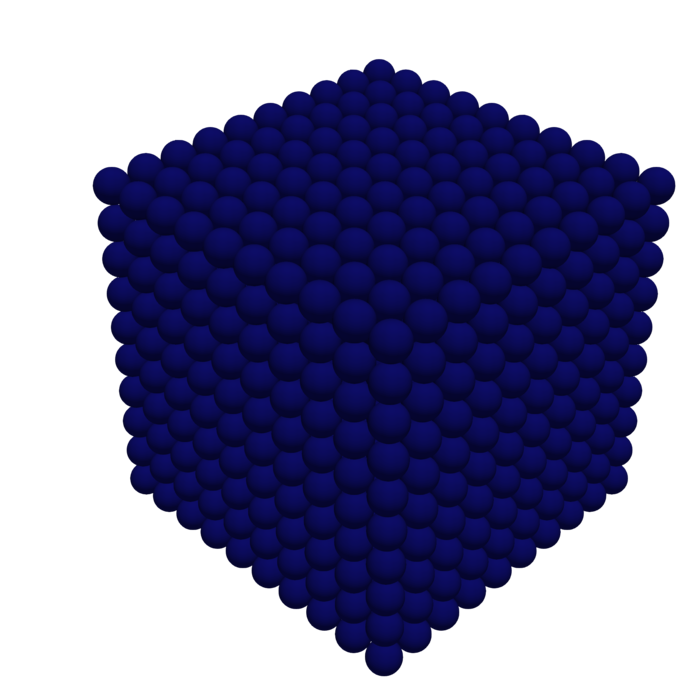
\includegraphics[width=\textwidth]{equilibrium/render/t0.png}
		\subcaption{Iteration \num{0}} % 0, 0
	\end{subfigure}%
	\begin{subfigure}[c]{.3\textwidth}
		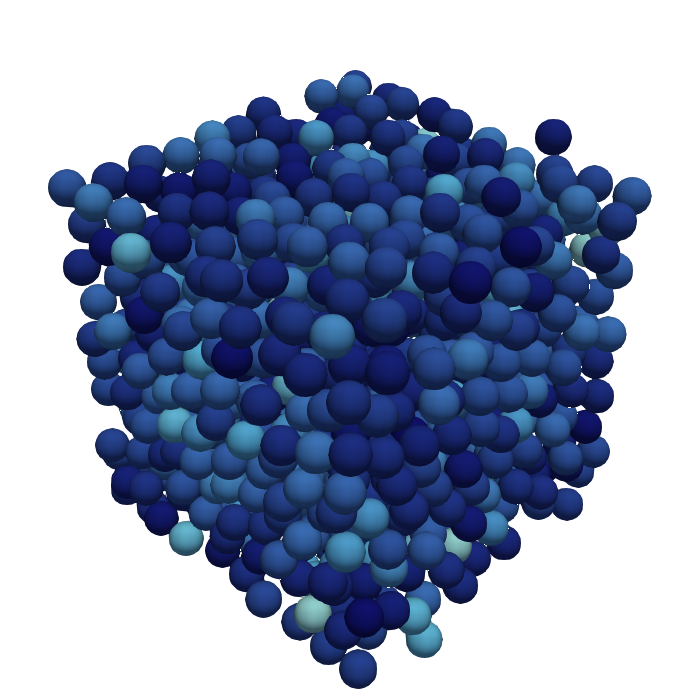
\includegraphics[width=\textwidth]{equilibrium/render/t10000.png}
		\subcaption{Iteration \num{10000}} % 10000, 10
	\end{subfigure}%
	\begin{subfigure}[c]{.3\textwidth}
		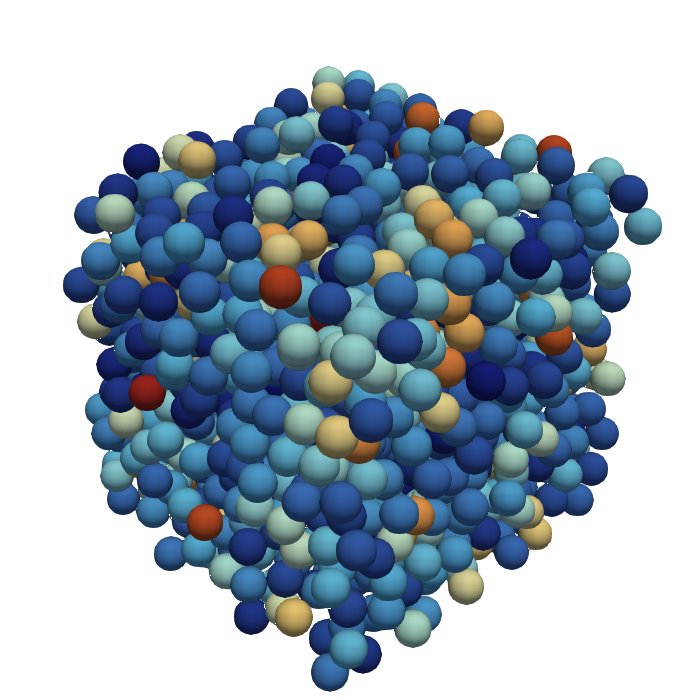
\includegraphics[width=\textwidth]{equilibrium/render/t50000.png}
		\subcaption{Iteration \num{50000}} % 50000, 50
	\end{subfigure}%
	\hfill\begin{subfigure}[c]{.08\textwidth}
		\fastcolorbar
	\end{subfigure}
	\caption{Evolution of the simulation state in the equilibrium scenario. The coloring indicates the forces acting upon a particle, and is given in reduced units.}
	\label{fig:evolution_equil}
\end{figure}


\subsection{Exploding Liquid}
Similarly to the equilibrium scenario, the exploding liquid scenario (\autoref{fig:evolution_expl}) starts of with the particles packed into a cuboid, with periodic boundaries applied to the simulation space. The cuboid explodes in $y$-direction and collides with the boundary. This leads to multiple waves of particles with decreasing intensity, until the simulation finally settles into an equilibrium state, with particles spread out over the whole domain. If a single autotuning instance is used for the whole domain, the rapid changes in particle positions and heterogeneous particle distribution make finding an optimal configuration very hard. However, if the domain is split up into multiple independent AutoPas instances on different MPI nodes, each AutoTuning instance can independently find an optimal configuration for its part of the domain. Using this, the simulation domain can be split up into regions with high particle density and velocities, and regions with little to no particles.

\label{subsec:expl}
\begin{figure}[htpb]
	\centering
	\begin{subfigure}[c]{.25\textwidth}
		\newsavebox{\colorbarbox}
		\savebox{\colorbarbox}{
			\fastcolorbarhor
		}
		\usebox{\colorbarbox}%
		\vspace*{-\ht\colorbarbox} %
		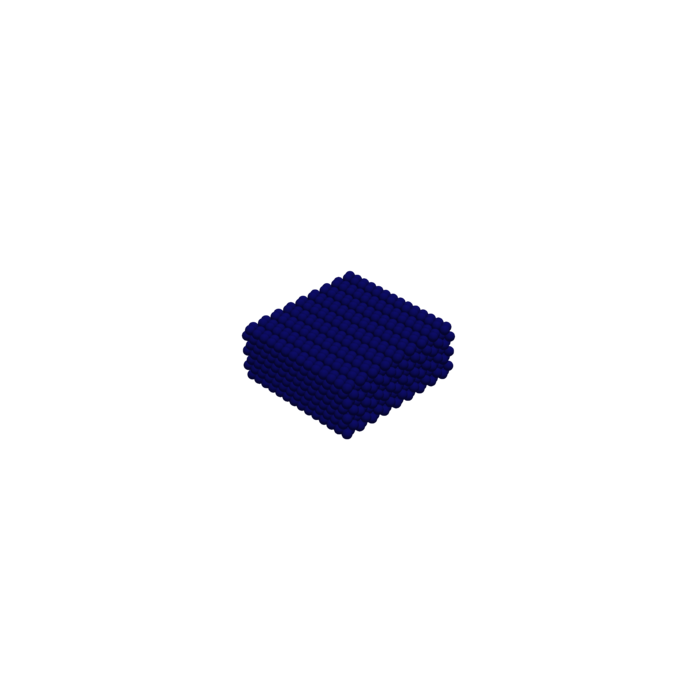
\includegraphics[width=\textwidth]{exploding-liquid/render/t0.png}
		\subcaption{Iteration \num{0}} % 0 
	\end{subfigure}%
	\begin{subfigure}[c]{.25\textwidth}
		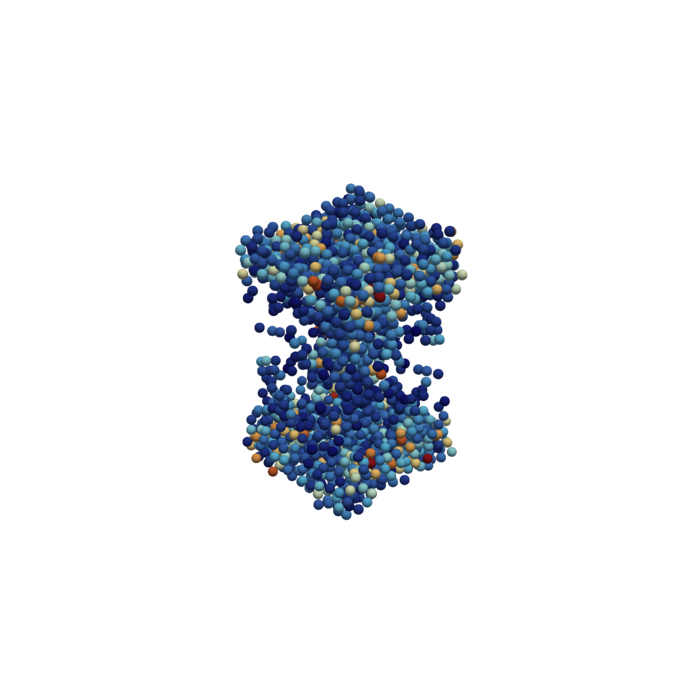
\includegraphics[width=\textwidth]{exploding-liquid/render/t3000.png}
		\subcaption{Iteration \num{3000}} % 3000, 5.5
	\end{subfigure}%
	\begin{subfigure}[c]{.25\textwidth}
		\centering
		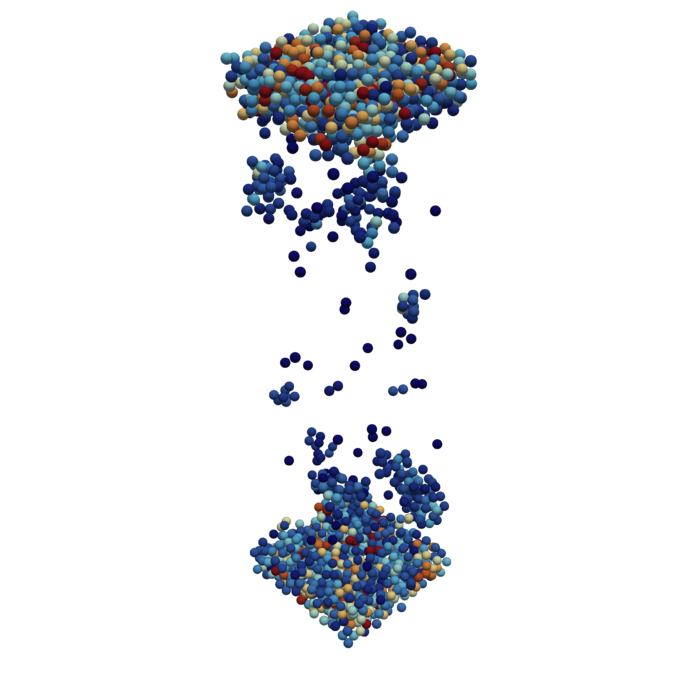
\includegraphics[width=\textwidth]{exploding-liquid/render/t11000.png}
		\subcaption{Iteration \num{11000}} % 11000, 20
	\end{subfigure}%
	\begin{subfigure}[c]{.25\textwidth}
		\centering
		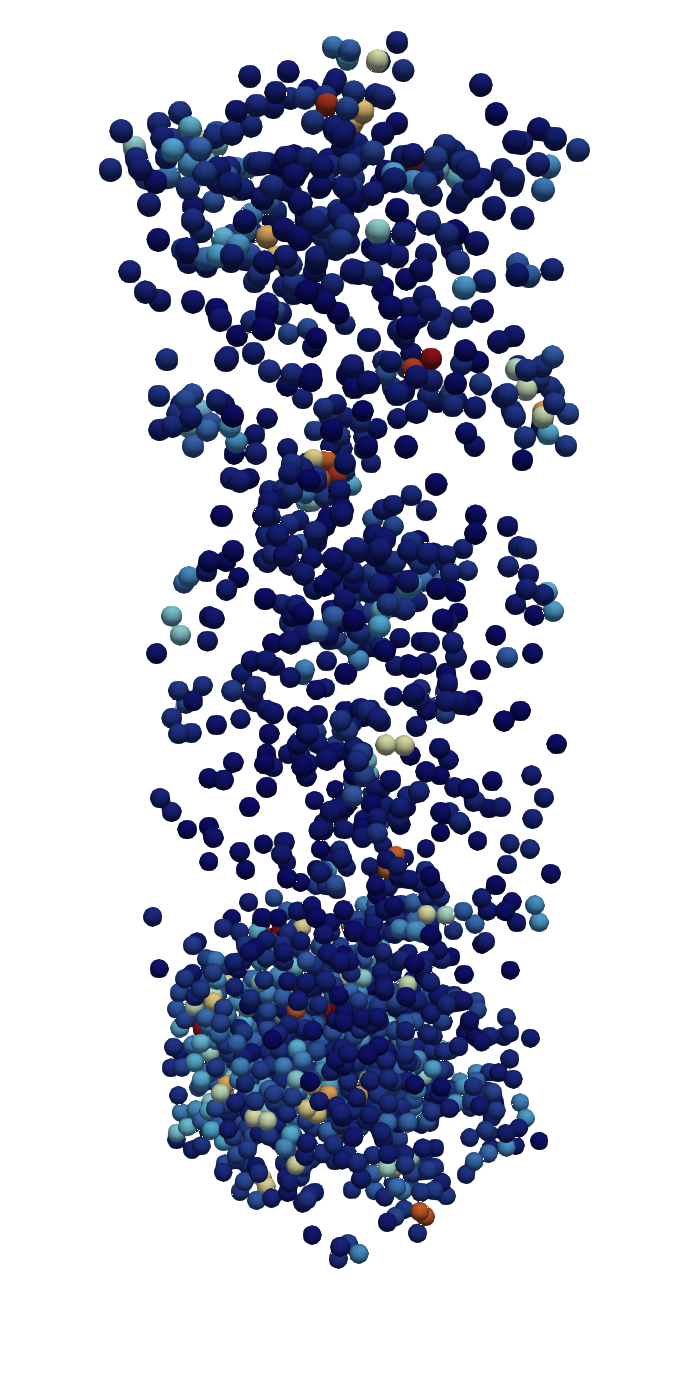
\includegraphics[width=\textwidth]{exploding-liquid/render/t31000.png}
		\subcaption{Iteration \num{31000}} % 31000, ?? 
	\end{subfigure}
	\caption{Evolution of the simulation state in the exploding liquid scenario.}
	\label{fig:evolution_expl}
\end{figure}

\subsection{Heating Sphere}
\label{subsec:hs}
The heating sphere scenario (\autoref{fig:evolution_hs}) starts off with a dense, small sphere of particles. In contrast to the previously introduced scenarios, reflective boundary conditions are applied. Over the course of the simulation, the temperature rises from $0.1$ to $100$ with a $\Delta \si{T^{*}}=0.1$ every 100 iterations. Additionaly, brownian motion, i.e. random fluctuations in particle positions, is applied \cite{Moerters2010}. The sphere expands with the increasing temperature and particles slowly radiate outwards. In the late phase of the simulation, particles are spread out across the whole domain.
Between the initial, compacted state and the equilibrated state, the optimal configuration changes.

\begin{figure}[htpb]
	\centering
	\fastcolorbarhor

	\begin{subfigure}[c]{.25\textwidth}
		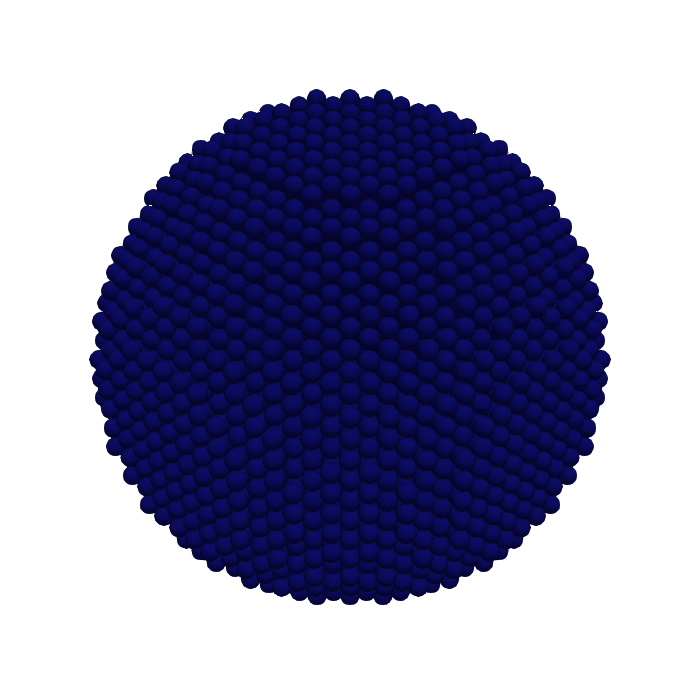
\includegraphics[width=\textwidth]{heating-sphere/render/t0.png}
		\subcaption{Iteration \num{0}} % 0
	\end{subfigure}%
	\begin{subfigure}[c]{.25\textwidth}
		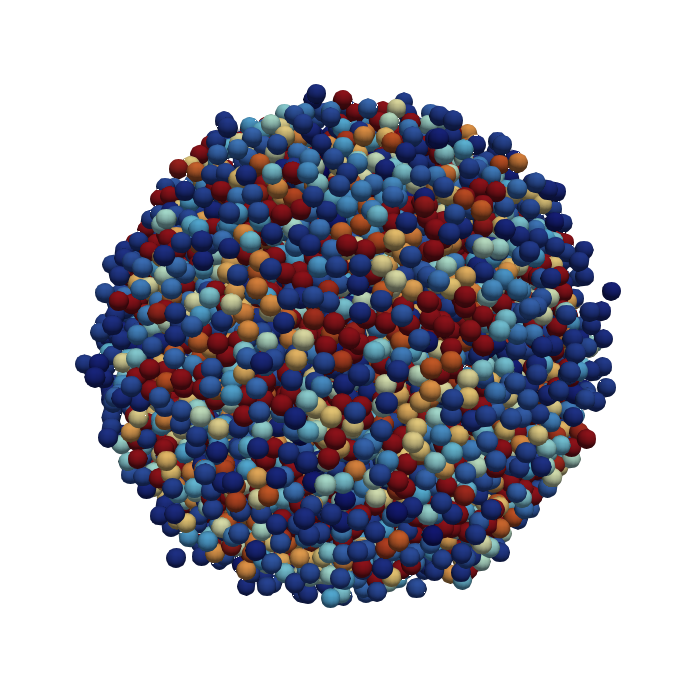
\includegraphics[width=\textwidth]{heating-sphere/render/t4000.png}
		\subcaption{Iteration \num{4000}} % 4000, 0.4
	\end{subfigure}%
	%		\begin{subfigure}[c]{.25\textwidth}
	%			\centering
	%			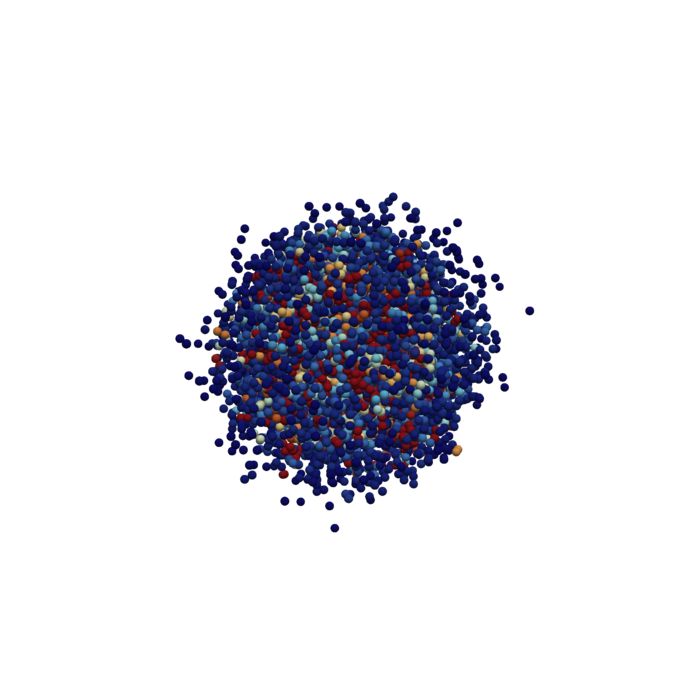
\includegraphics[width=\textwidth]{heating-sphere/render/t12000.png}
	%			\subcaption{Iteration \num{12000}} % 12000, 1.2
	%		\end{subfigure}%
	%	\hspace*{.15\textwidth} 
	\begin{subfigure}[c]{.25\textwidth}
		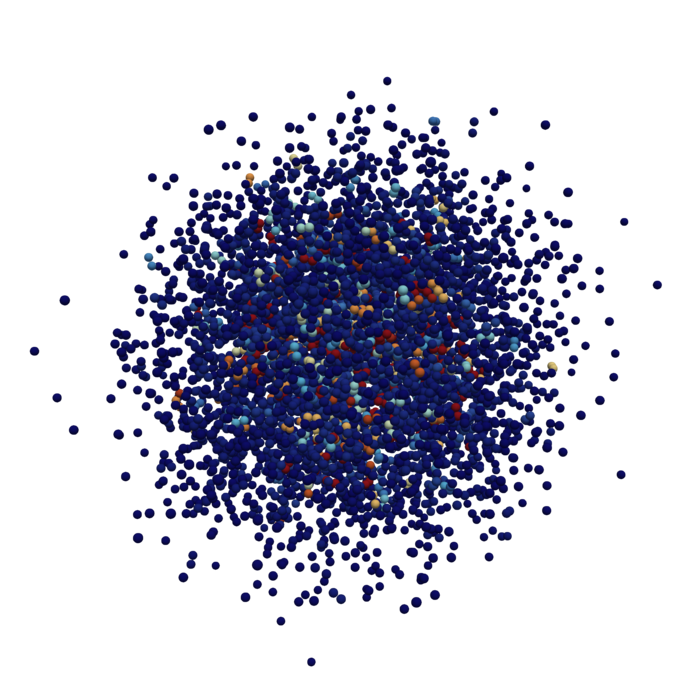
\includegraphics[width=\textwidth]{heating-sphere/render/t23000.png}
		\subcaption{Iteration \num{23000}} % 23000, 2.3
	\end{subfigure}%
	\begin{subfigure}[c]{.25\textwidth}
		\vspace*{0.1\textwidth}
		\centering
		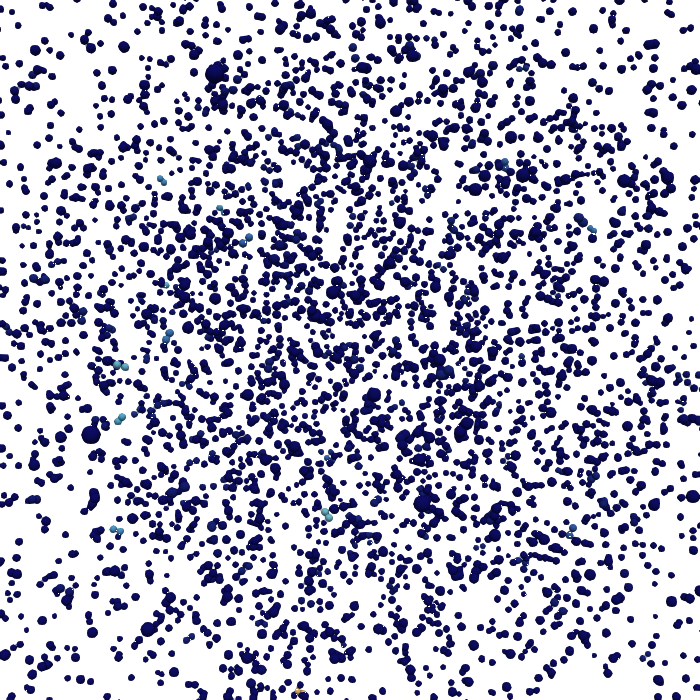
\includegraphics[width=0.8\textwidth]{heating-sphere/render/t60000.png}
		\vspace*{0.1\textwidth}
		\subcaption{Iteration \num{60000}} % 60000, 6
	\end{subfigure}%
	\caption{Evolution of the simulation state in the heating sphere scenario.}
	\label{fig:evolution_hs}
\end{figure}

%\subsection{Falling Drop}
%\label{subsec:fd}
%\subsection{Spinodial Decomposition}
%\label{subsec:sd}

\section{Evaluation Metrics}
\label{sec:metrics}
To compare results between dynamic and static tuning intervals, we use multiple metrics.
The primary goal is to reduce the total simulation runtime for a range of typical scenarios; it is therefore our primary metric. As tuning phases spend time in quite suboptimal configurations, a reduction in total runtime is the expected result if our approach reduces the number of tuning phases without spending too many iterations using a suboptimal configuration outside tuning phases.

% TODO: check this:
The metric of total runtime is not particularly fine-grained however, as it only takes into account entire simulation runs. To achieve a more detailed benchmark, we also consider the number of iterations that were computed under the optimal configuration. As an approximation to the optimal configuration in each iteration, we use simulation runs with tuning phases at fixed frequency, a high number of tuning samples and short tuning intervals. Based on this approximation we can then rank the configuration our dynamic run chose in terms of optimality.

Finally, we also consider the number of tuning phases initiated or, more precisely, the number of tuning iterations over the course of the whole simulation. Otherwise, we could not differentiate wether any achieved speedup is due to our trigger strategies or the fact that not triggering any tuning phases at all was more efficient for a given scenario.

\section{Default Trigger Parameters}
\label{sec:default_params}
% TODO: move to results?
All presented trigger strategies are based on a \texttt{trigger-factor} $\lambda$. The averaging, split and regression triggers additionally take into account the number of samples to inspect, denoted as $n$. For any dynamic tuning trigger to be useful, reasonable default values for these parameters are needed, as the performance of the whole simulation is dependent on the trigger's behavior.
Furthermore, optimal values for these parameters may depend on the scenario, trigger strategy or both.
These default values can be found by comparing a range of combinations $\left(\lambda_i, n_j\right)$ for any given scenario and trigger strategy.



\chapter[Results]{Results}
\label{cp:results}

{
	\parindent0pt
	\textellipsis
}

% How do results differ based on tuning strategy? Full-search vs. others
%TODO: make capitalization in titles consistent?

\section{Trigger Parameters}
% TODO: compare trigger factors and intervals
All presented trigger strategies are based on a trigger factor $\lambda$. The averaging, split and regression triggers additionally take into account the number of samples to inspect, denoted as $n$. For any dynamic tuning trigger to be useful, sensible default values for these parameters are needed, as the performance of the whole simulation is dependent on the trigger's behavior.

Therefore, we first inspect the relation between these parameters and the total simulation runtime for a range of combinations to find suitable default parameters for further evaluation.

\tikzset{
	linestyleA/.style={chaptertumblue, densely dotted, thick},
	linestyleB/.style={tumblueaccdark, densely dashed, thick},
	linestyleC/.style={tumblueaccmedium, solid, thick},
	linestyleD/.style={tumblueacclight, densely dashdotted, thick},
}

\pgfplotsset{
	triggerplot/.style={
			height=0.7\textwidth,
			width=\textwidth,
			xlabel={Trigger Factor $\lambda$},
			xtick={1.25, 1.5, 1.75},
			legend style={font=\small},
			legend cell align=center,
			legend columns=3,
			legend style={at={(0.5,1.03)}, anchor=south, fill=none, draw=none, align=center},
			legend image post style={xscale=0.5},
			ylabel near ticks},
	logtriggerplot/.style={
			triggerplot,
			log basis y = 10,
			log ticks with fixed point}
}

\subsection{Equilibrium}

\begin{figure}[htpb]
	\centering
	\begin{subfigure}{0.45\textwidth}
		\begin{tikzpicture}
			\begin{axis}[
					triggerplot,
					legend columns=2,
					ylabel={Speedup \%},
				]
				% TimeBasedSimple
				\addplot[linestyleD] coordinates{
						(1.25,-5)
						(1.5,12)
						(1.75,5)};
				% TimeBasedAverage 1000
				\addplot[linestyleA] coordinates{
						(1.25,21)
						(1.5,44)
						(1.75,47)};
				% TimeBasedAverage 500
				\addplot[linestyleB] coordinates{
						(1.25,10)
						(1.5,34)
						(1.75,47)};
				% TimeBasedAverage 250
				\addplot[linestyleC] coordinates{
						(1.25,17)
						(1.5,26)
						(1.75,34)};
				\legend{Simple,Avg-1000,Avg-500,Avg-250}
			\end{axis}
		\end{tikzpicture}
		%		\subcaption{Simple and Average Triggers}
	\end{subfigure}
	\hspace{0.05\textwidth}
	\begin{subfigure}{0.45\textwidth}
		\begin{tikzpicture}
			\begin{axis}[
					logtriggerplot,
					legend columns=2,
					ylabel={Tuning Iterations \%},
					ymode=log,
					ymin=1,
					ymax=100,
				]
				% TimeBasedSimple
				\addplot[tumblueacclight, thick] coordinates{
						(1.25,29.37)
						(1.5,2.26)
						(1.75,2.26)};
				% TimeBasedAverage 1000
				\addplot[linestyleA] coordinates{
						(1.25,2.26)
						(1.5,1.51)
						(1.75,1.51)};
				% TimeBasedAverage 500
				\addplot[linestyleB] coordinates{
						(1.25,2.26)
						(1.5,2.26)
						(1.75,1.51)};
				% TimeBasedAverage 250
				\addplot[linestyleC] coordinates{
						(1.25,2.26)
						(1.5,1.51)
						(1.75,1.51)};
				\legend{Simple,Avg-1000,Avg-500,Avg-250}
			\end{axis}
		\end{tikzpicture}
		%		\subcaption{Simple and Average Triggers}
	\end{subfigure}
	\begin{subfigure}{0.45\textwidth}
		\begin{tikzpicture}
			\begin{axis}[
					triggerplot,
					ylabel={Speedup \%},
				]
				% TimeBasedSplit 1000
				\addplot[linestyleA] coordinates{
						(1.25,42)
						(1.5,46)
						(1.75,35)};
				% TimeBasedSplit 500
				\addplot[linestyleB] coordinates{
						(1.25,43)
						(1.5,38)
						(1.75,40)};
				% TimeBasedSplit 250
				\addplot[linestyleC] coordinates{
						(1.25,-6)
						(1.5,28)
						(1.75,-7)};
				\legend{Split-1000,Split-500,Split-250}
			\end{axis}
		\end{tikzpicture}
		%		\subcaption{Split Trigger}
	\end{subfigure}
	\hspace{0.05\textwidth}
	\begin{subfigure}{0.45\textwidth}
		\begin{tikzpicture}
			\begin{axis}[
					logtriggerplot,
					ylabel={Tuning Iterations \%},
					ymode=log,
					ymin=1,
					ymax=100,
				]
				% TimeBasedSplit 1000
				\addplot[linestyleA] coordinates{
						(1.25,3.77)
						(1.5,3.01)
						(1.75,3.77)};
				% TimeBasedSplit 500
				\addplot[linestyleB] coordinates{
						(1.25,4.52)
						(1.5,4.52)
						(1.75,3.77)};
				% TimeBasedSplit 250
				\addplot[linestyleC] coordinates{
						(1.25,81.7)
						(1.5,6.03)
						(1.75,81.9)};
				\legend{Split-1000,Split-500,Split-250}
			\end{axis}
		\end{tikzpicture}
		%		\subcaption{Split Trigger}
	\end{subfigure}
	\begin{subfigure}{0.45\textwidth}
		\begin{tikzpicture}
			\begin{axis}[
					triggerplot,
					ylabel={Speedup \%},
				]
				% TimeBasedRegression 2000
				\addplot[linestyleA] coordinates{
						(1.25,46)
						(1.5,33)
						(1.75,34)};

				% TimeBasedRegression 1500
				\addplot[linestyleB] coordinates{
						(1.25,46)
						(1.5,46)
						(1.75,31)};
				% TimeBasedRegression 1000
				\addplot[linestyleC] coordinates{
						(1.25,43)
						(1.5,44)
						(1.75,44)};

				\legend{Reg-2000,Reg-1500,Reg-1000}
			\end{axis}
		\end{tikzpicture}
		%		\subcaption{Regression Trigger}
	\end{subfigure}%
	\hspace{0.05\textwidth}
	\begin{subfigure}{0.45\textwidth}
		\begin{tikzpicture}
			\begin{axis}[
					logtriggerplot,
					ylabel={Tuning Iterations \%},
					%ymode=log,
					ymin=0,
					ymax=1,
					ytick={0, 0.25, 0.75, 1.0},
				]
				% TimeBasedRegression 2000
				\addplot[linestyleA] coordinates{
						(1.25,0.75)
						(1.5,0.75)
						(1.75,0.75)};

				% TimeBasedRegression 1500
				\addplot[linestyleB] coordinates{
						(1.25,0.75)
						(1.5,0.75)
						(1.75,0.75)};
				% TimeBasedRegression 1000
				\addplot[linestyleC] coordinates{
						(1.25,0.75)
						(1.5,0.75)
						(1.75,0.75)};

				\legend{Reg-2000,Reg-1500,Reg-1000}
			\end{axis}
		\end{tikzpicture}
		%		\subcaption{Regression Trigger}
	\end{subfigure}%
	\caption{Trigger behavior in the equilibrium scenario, the numbers in the legends refer to the number of samples $n$ considered. Note the logarithmic scale in the plots for the tuning iterations.}
	\label{fig:params_equil}
\end{figure}

As can be seen in \autoref{fig:params_equil}, a trigger factor of $\lambda=1.5$ leads to increased speedup compared to $\lambda=1.25$. This is however mainly due to the nature of the equilibrium scenario: after the initial configuration selection, the optimal configuration is not expected to change.
Therefore, not initiating any new tuning phases will lead to a decrease in total simulation runtime. That the speedup is indeed  a result of the decreased number of tuning iterations can be verified by looking at the right-hand side plots; for the simple and averaging trigger it is most noticeable.
Additionally, triggers with a larger sample size will typically trigger less frequently, as more of the variability in iteration runtime is smoothed out. For a too large number of samples, the speedup decreases however, computational overhead is directly proportional to the number of samples. This is best seen in the plots for the regression trigger, as the share of tuning iterations remains constant for all sample sizes, but the speedup decreases. Especially for the regression triggers, the computations required per sample and in each iteration are significant.
%The increase of th enumber of tuning iterations as seen in the split trigger with $n=250$ can be explained by \textellipsis
% TODO: self-interaction

The collected data suggests default parameters as presented in \autoref{tab:equil_defaults}.
\begin{table}[htpb]
	\centering
	\begin{tabular}{lcc}
		\toprule
		\textbf{Trigger}                      & \textbf{Trigger factor $\lambda$} & \textbf{Number of samples $n$} \\ [0em]
		\midrule
		\texttt{TimeBasedSimple}     & $1.75$                   & --                     \\
		\texttt{TimeBasedAverage}    & $1.75$                   & 500                   \\
		\texttt{TimeBasedSplit}      & $1.5$                    & 1000                  \\
		\texttt{TimeBasedRegression} & $1.5$                    & 1500                  \\
		\bottomrule
	\end{tabular}
	\caption{Suggested default parameters for the equilibrium scenario.}
	\label{tab:equil_defaults}
\end{table}

\subsection{Exploding Liquid}
\subsection{Heating Sphere}

\section{Trigger Behavior}
The blue bars in the graphs represent the runtime of that particular iteration.
In the configuration plots, the colored background identifies the used configuration: same configurations map to the same color. The gaps in the plot are where tuning iterations have been logged -- as their runtime is not relevant for the scenario change and would distort the actual runtime plot, they are not reported here. The red vertical lines indicate the start of a tuning phase.

\subsection{Simple Trigger}
\subsection{Single-iteration averaging Trigger}
\subsection{Interval averaging Trigger}
\subsection{Linear Regression Trigger}


\section{Optimality}
\section{Runtime}
\section{Share of Tuning Iterations}


\chapter[Conclusion]{Conclusion}
\label{cp:conclusion}

\vspace*{-2ex} % TODO: check alignment
In this thesis, four new methods to dynamically initiate new tuning phases in AutoPas were introduced. Additionally, reasonable default values for the corresponding control parameters were derived empirically.
It was shown that our trigger strategies decrease simulation runtime across almost all tested scenarios when using \texttt{full-search} as the tuning strategy. % TODO: average speedup across all
Especially in settings with low variance in iteration runtime, all strategies reduce the number of iterations spent in tuning phases without any significant decrease in the optimality of the used configurations. %TODO: check this
The most promising candidate was shown to be the comparison of averaged intervals, due to its resilience to noise in the live input data, leading to speedups of up to \qty{76}{\percent} under optimal conditions.
The other strategies investigated are more susceptible to the aforementioned fluctuations in the input data. Nonetheless, these triggers still perform well in scenarios with low variance between iterations. % TODO

However, as new tuning strategies are introduced, the dynamic initiation of tuning intervals will likely become less relevant for single-node applications. In particular, tuning strategies based on machine learning lead to cheap tuning phases \cite{Newcome2025}, which in turn significantly diminishes the achievable speedups. One application in which a dynamic approach as ours might still be of use, is in distributed memory setups: As each node runs its own AutoPas instance, it can trigger tuning phases independently from other nodes. In scenarios with heterogeneous particle distribution over the whole domain, the best configuration on a specific node is likely to change separate from other parts of the domain. Thus, our proposed method may still be advantageous.

Possible future work may explore the analysis of additional live simulation statistics, either as single parameter or hybrid strategies. The introduction of novel triggering algorithms providing more stability, such as linear regression using the Theil-Sen estimator, should be considered. More advanced methods such as digital filters have to be implemented efficiently, as not to inflate per-iteration overhead.
Another interesting subject for further research could be the combination of static and dynamic tuning intervals; at fixed, but much shorter intervals, a dynamic trigger would evaluate whether to start a new tuning phase or not.

% TODO: check if lightweight
In summary, the dynamic initiation of tuning phases has been shown to be lightweight method of decreasing unnecessary tuning phases, whilst still ensuring good configuration fit. Using more efficient tuning strategies reduces the performance gains in single-node applications, but some benefits remain in multi-node settings.


%%% Bibliography %%%
\renewcommand{\refname}{Bibliography}
\printbibliography[title={\refname},heading=bibintoc]

%%% Appendices: Work that *YOU* Developed %%%
%\appendix
%\ifthenelse{\equal{\LanguageOption}{portuguese}}{
    \addtocontents{toc}{\protect\contentsline{chapter}{Apêndices}{}{}}
}{
    \addtocontents{toc}{\protect\contentsline{chapter}{Appendices}{}{}}
}

\ifthenelse{\equal{\MediaOption}{paper}}{\blankpage}{\clearpage}
\begin{center}
    \thispagestyle{empty}
        
    \vspace*{\fill}
    \ifthenelse{\equal{\LanguageOption}{portuguese}}{%
        {\LARGE\fontsize{26}{26}\selectfont\textcolor{maincolor}{Apêndices}\par}
    }{%
        {\LARGE\fontsize{26}{26}\selectfont\textcolor{maincolor}{Appendices}\par}
    }
    \vspace*{\fill}
\end{center}
\MediaOptionLogicBlank
%\chapter{Showcasing the First Appendix}
\guideinfo{Appendices contain supplementary material \textbf{created by the author} that enhances the reader’s understanding of the dissertation while not being essential for following the primary narrative. These sections often include detailed tables, figures, complex calculations, or materials like survey questions and interview transcripts produced in the course of the research. The appendices allow readers to explore the research in greater detail, offering a deeper insight into methods and findings without interrupting the main body of work.}
%% Recommended dimensions for a landscape layout; adjust as needed.
\begin{landscapemode}{297mm}{420mm}
    \chapter{Showcasing the Second Appendix}
    \blindtext[5]
\end{landscapemode}

%%% Annexes: Work that *YOU DID NOT* Develop %%%
%\ifthenelse{\equal{\LanguageOption}{portuguese}}{
    \addtocontents{toc}{\protect\contentsline{chapter}{Anexos}{}{}}
}{
    \addtocontents{toc}{\protect\contentsline{chapter}{Annexes}{}{}}
}

\setcounter{chapter}{11} % To start at the "L" chapter.
\MediaOptionLogicAnnexes
\begin{center}
    \minionfont
    \thispagestyle{empty}
        
    \vspace*{\fill}
    \ifthenelse{\equal{\LanguageOption}{portuguese}}{%
        {\LARGE\fontsize{26}{26}\selectfont\textcolor{maincolor}{Anexos}\par}
    }{%
        {\LARGE\fontsize{26}{26}\selectfont\textcolor{maincolor}{Annexes}\par}
    }
    \vspace*{\fill}
\end{center}
\MediaOptionLogicBlank
%\chapter{Showcasing the First Annex}
\guideinfo{Annexes are supplementary sections in a dissertation that provide additional information or external documents not essential to the main arguments but that support or complement the research. Unlike appendices, \textbf{annexes generally contain material that was not developed by the author}, such as reports, legal documents, or published datasets from external sources. This information is placed separately to keep the main content concise, allowing readers access to relevant external references without disrupting the dissertation's flow.}

%%% Back Page %%%
\ifthenelse{\equal{\MediaOption}{paper}}{\blankpage}{}

\clearpage
\null
\thispagestyle{empty}

\ifthenelse{\equal{\CoverOption}{classic}}{
    \newcommand\BackgroundPicBackPage{%
    \put(0,0){%
    \parbox[b][\paperheight]{\paperwidth}{%
    \vfill
    \centering
    
\includegraphics[width=\paperwidth,height=\paperheight,keepaspectratio]{Figures/Theme/Back-Page-BG.pdf}%
    \vfill
    }}}
}{
    \newcommand\BackgroundPicBackPage{%
    \put(0,0){%
    \parbox[b][\paperheight]{\paperwidth}{%
    \vfill
    \centering
    
\includegraphics[width=\paperwidth,height=\paperheight,keepaspectratio]{Figures/Theme/Back-Page-BG-W.pdf}%
    \vfill
    }}}
}

\AddToShipoutPictureBG*{\BackgroundPicBackPage}

\newgeometry{margin=1.98cm, top=1.47cm, bottom=1.47cm}
\noindent\clearpage
\restoregeometry

\end{document}